

\documentclass [PhD] {uclathes}

\newcommand{\minsum}{Min Sum}

%channel
\newcommand{\y}{\mathbf{y}}
\newcommand{\x}{\mathbf{x}}
\newcommand{\xel}{x}
\newcommand{\xalph}{\mathcal{X}}
\newcommand{\yalph}{\mathcal{Y}}
\newcommand{\noisestd}{\sigma}
\newcommand{\snr}{\mathrm{SNR}}
\newcommand{\dabpmf}{p_{\mathrm{DAB}}}
%message and CRC
\newcommand{\numbits}{k}
\newcommand{\alabelel}{w}
\newcommand{\alabel}{\mathbf{\alabelel}}
\newcommand{\crcquotel}{q}
\newcommand{\crcquot}{\mathbf{\crcquotel}}
\newcommand{\ceq}{\mathbf{G}_{\mathrm{eq}}}
\newcommand{\peq}{\mathbf{P}_{\mathrm{eq}}}
\newcommand{\convc}{\mathbf{G}}
%convolutional encoder
\newcommand{\length}{l}
\newcommand{\uinel}{u}
\newcommand{\uin}{\mathbf{\uinel}}
\newcommand{\convrate}{k}
%Pairwise Error probability
\newcommand{\FER}{\mathrm{FER}}
\newcommand{\pairwiseerrorevent}[1]{\mathbf{e}_{#1}}
%codeword indices; renew when section uses different ones
\newcommand{\corridx}{c}
\newcommand{\erridx}{e}
\newcommand{\errorevent}{\varepsilon_{\mathbf{x}_c}}
\newcommand{\PEE}{e_{\mathbf{x}_c,\mathbf{x}_e}}
\newcommand{\PEP}{P\left(\PEE\right)}
%modified metric
\newcommand{\xc}{\x_{\corridx}}%correct codeword
\newcommand{\xe}{\x_{\erridx}}%incorrect codeword
\newcommand{\uc}{\uin_{\corridx}}%correct codeword
\newcommand{\ue}{\uin_{\erridx}}%incorrect codeword
\newcommand{\yprime}{\mathbf{z}'}
\newcommand{\dplain}{d}
\newcommand{\de}{d_{\mathrm{E}}}
\newcommand{\dnew}{d_{\mathrm{new}}}
\newcommand{\da}{d_{\mathrm{prox}}}
%transfer function
\newcommand{\dfree}{d_{\mathrm{free}}}
\newcommand{\overell}{_{\ell = 1}^\length}
% \newcommand{\errstate}{s}
% \newcommand{\encstate}{r}
% \newcommand{\errstatevec}{\mathbf{\errstate}}
% \newcommand{\encstatevec}{\mathbf{\encstate}}
\newcommand{\eq}{{q}}
\newcommand{\err}{e}
\newcommand{\errstart}{s_\err}
\newcommand{\errend}{s'_\err}
\newcommand{\eqstart}{s_\eq}
\newcommand{\eqend}{s'_\eq}
\newcommand{\erri}{\err_i}
\newcommand{\erro}{\err_o}
\newcommand{\tbcc}{T_{\mathrm{TBCC}}}
\newcommand{\errcnt}{\mathcal{S}_\err}
\newcommand{\eqcnt}{\mathcal{S}_\eq}
%matrices
\newcommand{\bigmat}{\mathbf{G}}
%misc
\newcommand{\reals}{\mathbb{R}}
\newcommand{\pmf}{PMF}
\newcommand{\setedge}{\mathcal{E}}
\newcommand{\setstate}{\mathcal{V}}
\newcommand{\interval}{\mathcal{I}}
\newcommand{\outlen}{n}


\newcommand{\equl}{\Tilde{l}}



%polynomials
\newcommand{\polyvar}{x}
\newcommand{\convpoly}{p(x)}
\newcommand{\uinpoly}{\uinel(\polyvar)}
\newcommand{\uinsplit}{\uin_{\mathrm{split}}(\polyvar)}
\newcommand{\crcquotsplit}{\crcquot_{\mathrm{split}}(\polyvar)}
\newcommand{\alabelsplit}{\alabel_{\mathrm{split}}(\polyvar)}




\newcommand{\soursymsqe}{\mathbf{s}}
\newcommand{\crcinb}{\mathbf{g}}
\newcommand{\crcoutb}{\mathbf{h}}
\newcommand{\crcins}{\mathbf{w}}
\newcommand{\cicous}{\mathbf{u}}
\newcommand{\dmou}{\mathbf{a}}
\newcommand{\chaninsy}{\mathbf{x}}


%%TBCC
\newcommand{\ccinnum}{k_0}
\newcommand{\ccoutnum}{\gamma_0}
\newcommand{\ccoutputset}{\mathcal{O}}
\newcommand{\ccoutputrealize}{o}



                         % personal LaTeX macros
%%-------Linfang Package------
\usepackage{graphicx}
\usepackage{epstopdf}
\usepackage[caption=false,font=footnotesize]{subfig}
\usepackage{cite}
\usepackage{color}
\usepackage{xcolor}
\usepackage[cmex10]{amsmath}
\usepackage{amssymb}
\usepackage{threeparttable}
\usepackage{mathtools}
\usepackage{hyperref}
\usepackage{algpseudocode}
\usepackage{multirow}
\usepackage[T1]{fontenc}
\usepackage[ruled]{algorithm2e}
\usepackage{booktabs}
\usepackage{stfloats}
\usepackage{tensor}
\usepackage{bbm}
\usepackage{multicol}
\usepackage{tikz}
\usepackage{cooltooltips}
\def\cool{\texttt{cool}}
\definecolor{mygreen}{rgb}{0.1,.6,0.1}
\DeclareMathOperator*{\argmax}{argmax} 
\DeclareMathOperator*{\argminB}{argmin}   % Jan Hlavacek
%%------Tikz Package------
\usepackage{tikz}
\usetikzlibrary{shapes.geometric, arrows}
\tikzstyle{startstop} = [rectangle, rounded corners, minimum width=3cm, minimum height=1cm,text centered, draw=black, fill=red!30]
\tikzstyle{io} = [trapezium, trapezium left angle=70, trapezium right angle=110, minimum width=3cm, minimum height=1cm, text centered, draw=black, fill=blue!30]
\tikzstyle{process} = [rectangle, minimum width=3cm, minimum height=1cm, text centered, draw=black, fill=orange!30]
\tikzstyle{decision} = [diamond, minimum width=3cm, minimum height=1cm, text centered, draw=black, fill=green!30]
\tikzstyle{arrow} = [thick,->,>=stealth]
\usetikzlibrary{calc}
\usepackage{relsize}
\usepackage{pgfplots}
\usetikzlibrary{plotmarks}
\usetikzlibrary{arrows}
\usetikzlibrary{spy,backgrounds}
\usepackage{tikz-3dplot}
\usetikzlibrary{positioning,chains,fit,shapes,calc}
\usetikzlibrary{pgfplots.groupplots}
\tikzset{fontscale/.style = {font=\relsize{#1}}}
\usepackage{amsthm}
\newtheorem{thm}{Theorem}
\newtheorem{lem}[thm]{Lemma}
\usepackage[ruled]{algorithm2e}
\pgfplotsset{table/search path={data}}
\pgfplotsset{compat=1.3}
\usepackage{ragged2e}
\newcommand\gauss[2]{1/(#2*sqrt(2*pi))*exp(-((x-#1)^2)/(2*#2^2))} 
\pgfplotsset{width=7cm,compat=1.15}
\usepackage{makecell}
\setcellgapes{2pt}
\usepackage[thinlines]{easytable}
\newcommand{\floor}[1]{\left\lfloor #1 \right\rfloor}
\newcommand{\ceil}[1]{\left\lceil #1 \right\rceil}
%%%%%%%%%%%%%%%%%%%%%%%%%%%%%%%%%%%%%%%%%%%%%%%%%%%%%%%%%%%%%%%%%%%%%%
%
% Usually things live in separate flies.
%
% \input {prelim}                           % preliminary page info

%%%%%%%%%%%%%%%%%%%%%%%%%%%%%%%%%%%%%%%%%%%%%%%%%%%%%%%%%%%%%%%%%%%%%%%%
%                                                                      %
%                          PRELIMINARY PAGES                           %
%                                                                      %
%%%%%%%%%%%%%%%%%%%%%%%%%%%%%%%%%%%%%%%%%%%%%%%%%%%%%%%%%%%%%%%%%%%%%%%%

\title          {Low-Complexity Decoding of Low-Density Parity Check Codes \\
                Through Optimal Quantization and Machine Learning \\
                and Optimal Modulation and Coding for Short Block-Length Transmissions}
\author         {Linfang Wang}
\department     {Electrical Engineering}
% Note:  degreeyear should be optional, but as of  5-Feb-96
% it seems required or you get a year of ``2''.   -johnh
\degreeyear     {2023}

%%%%%%%%%%%%%%%%%%%%%%%%%%%%%%%%%%%%%%%%%%%%%%%%%%%%%%%%%%%%%%%%%%%%%%%%

\member         {Christina Fragouli}
\member         {Dariush Divsalar}
\member         {Gregory J.\ Pottie}
\member         {Lara Dolecek}
\chair          {Richard D.\ Wesel}

%%%%%%%%%%%%%%%%%%%%%%%%%%%%%%%%%%%%%%%%%%%%%%%%%%%%%%%%%%%%%%%%%%%%%%%%


 
\dedication     {\textsl{To my parents, Genqi and Xiangqun \ldots \\
                To my wife, my dear Hanzhi (Stephanie) \ldots \\}}

%%%%%%%%%%%%%%%%%%%%%%%%%%%%%%%%%%%%%%%%%%%%%%%%%%%%%%%%%%%%%%%%%%%%%%%%

\acknowledgments {(Acknowledgments omitted for brevity.)}

%%%%%%%%%%%%%%%%%%%%%%%%%%%%%%%%%%%%%%%%%%%%%%%%%%%%%%%%%%%%%%%%%%%%%%%%

\vitaitem   {1974--1975}
                {Campus computer center ``User Services'' programmer and
                consultant, Stanford Center for Information Processing,
                Stanford University, Stanford, California.}
\vitaitem   {1974--1975}
                {Programmer, Housing Office, Stanford University.
                Designed a major software system for assigning
                students to on-campus housing.
                With some later improvements, it is still in use.}
\vitaitem   {1975}
                {B.S.~(Mathematics) and A.B.~(Music),
                Stanford University.}
\vitaitem   {1977}
                {M.A.~(Music), UCLA, Los Angeles, California.}
\vitaitem   {1977--1979}
                {Teaching Assistant, Computer Science Department, UCLA.
                Taught sections of Engineering 10 (beginning computer
                programming course) under direction of Professor Leon
                Levine.
                During summer 1979, taught a beginning programming
                course as part of the Freshman Summer Program.}
\vitaitem   {1979}
                {M.S.~(Computer Science), UCLA.}
\vitaitem   {1979--1980}
                {Teaching Assistant, Computer Science Department, UCLA.}
\vitaitem   {1980--1981}
                {Research Assistant, Computer Science Department, UCLA.}
\vitaitem   {1981--present}
                {Programmer/Analyst, Computer Science Department, UCLA.}

%%%%%%%%%%%%%%%%%%%%%%%%%%%%%%%%%%%%%%%%%%%%%%%%%%%%%%%%%%%%%%%%%%%%%%%%

\publication    {\textsl{MADHOUS Reference Manual.}
                Stanford University, Dean of Student Affairs
                (Residential Education Division), 1978.
                Technical documentation for the MADHOUS
                software system used to assign students to
                on-campus housing.}

%%%%%%%%%%%%%%%%%%%%%%%%%%%%%%%%%%%%%%%%%%%%%%%%%%%%%%%%%%%%%%%%%%%%%%%%

\abstract       {(Abstract omitted for brevity)}

%%%%%%%%%%%%%%%%%%%%%%%%%%%%%%%%%%%%%%%%%%%%%%%%%%%%%%%%%%%%%%%%%%%%%%%%



\begin {document}
\makeintropages

%%%%%%%%%%%%%%%%%%%%%%%%%%%%%%%%%%%%%%%%%%%%%%%%%%%%%%%%%%%%%%%%%%%%%%
%
% Ordinarily each chapter (at least) is in a separate file.
%
%\input {chapter1}                         % Chapter 1 of dissertation
%\input {chapter2}                         % Chapter 2
%\input {chapter3}                         % etc.
%\input {chapter4}
%\input {chapter5}
%\input {chapter6}
%\input {chapter7}
%\input {chapter8}

\chapter{Introduction}

For text, let's use the first words out of the ispell dictionary.



\chapter{Reconstruction-Computation-Quantization (RCQ): A Paradigm for Low Bit Width LDPC Decoding}


\section{Introduction}
Low-Density Parity-Check  (LDPC) codes \cite{GallagerPhD1963} have been implemented broadly, including in NAND flash systems and wireless communication systems. Message passing algorithms such as belief propagation (BP) and \minsum are utilized in LDPC decoders. In practice, decoders with low message bit widths are desired when considering the limited hardware resources such as area, routing capabilities, and power utilization of FPGAs or ASICs. Unfortunately, low bit width decoders with uniform quantizers typically suffer a large degradation in decoding performance\cite{-_Lee2005-MIMQBP}. On the other hand, the iterative decoders that allow for the dynamic growth of message magnitudes can achieve improved performance\cite{Zhang2014-ib}.




%----FAID--------
LDPC decoders that quantize messages  non-uniformly have gained attention because they provide excellent decoding performance with low bit width message representations. 
One family of non-uniform LDPC decoders use lookup tables (LUTs) to replace the mathematical operations in the check node (CN) unit  and/or the variable node (VN) unit. 
%\textcolor{red}{The LUTs are built based on non-uniform quantizers for the decoder.} 
S. K. Planjery \emph{et al.} propose finite alphabet iterative decoders (FAIDs) for regular LDPC codes in \cite{Planjery2013-FAIDI,Declercq2013-FAIDII},  which optimize a \textit{single} LUT to describe VN input/output behavior. In \cite{Planjery2013-FAIDI} a FAID is  designed to tackle certain trapping sets and hence achieves a lower error floor than BP on the binary symmetric channel (BSC).  Xiao \emph{et al.} optimize the parameters of FAID using a recurrent quantized neural network (RQNN)\cite{Xiao2019-RNNFIAD,Xiao2020-RNNFAID}, and the simulation results show that RQNN-aided linear FAIDs are capable of surpassing floating-point BP in the waterfall region for regular LDPC codes.

%----MIMQBP----
Note that the size of the LUTs in \cite{Planjery2013-FAIDI,Declercq2013-FAIDII,Xiao2019-RNNFIAD,Xiao2020-RNNFAID} describing VN behavior are an exponential function with respect to node degree. Therefore, these FAIDs can only handle regular LDPC codes with small node degrees. For codes with large node degrees, Kurkoski {\em et al}. develop a mutual-information-maximization LUT (MIM-LUT) decoder in \cite{kurkoski2016-IB}, which decomposes a single LUT with multiple inputs into a series of concatenated $2\times1$ LUTs, each with two inputs and one output. This decomposition makes the number of LUTs linear with respect to node degree, thus significantly reducing the required memory.  The MIM-LUT decoder performs lookup operations at both the CNs and VNs. The 3-bit MIM-LUT decoder shows a better FER than floating-point BP over the additive white Gaussian noise (AWGN) channel. As the name suggests, the individual $2\times1$ LUTs are designed to maximize mutual information\cite{Kurkoski2014-QuanDMC}.   

%----IB Decoder------
Lewandowsky \emph{et al.} use the information bottleneck (IB) machine learning method to design LUTs and propose an IB decoder for regular LDPC codes. As with MIM-LUT, IB decoders also use $2\times1$ LUTs at both CNs and VNs. Stark \emph{et al.} extend the IB decoding structure to support irregular LDPC codes through the technique of message alignment \cite{Stark2018-IBMA,Stark2021-ai}. 
The IB decoder shows an excellent performance on a 5G LDPC code\cite{Stark2020-IB5G,Stark2020-IBjournal}. In order to reduce the memory requirement for LUTs, Meidlinger \emph{et al.} propose the Min-IB decoder, which replaces the LUTs at CNs with label-based min operation \cite{Meidlinger2015-MIMIB,Meidlinger2017-MINIBIRR,Meidlinger2020-MINIBIRR,Ghanaatian2018-MINIB-588}.


Because the decoding requires only simple lookup operations, the LUT-based decoders deliver high throughput. However, the LUT-based decoders require significant memory resources when the LDPC code has large degree nodes and/or the decoder has a large predefined maximum decoding iteration time, where each iteration requires its own LUTs. The huge memory requirement for numerous large LUTs prevents these decoders from being viable options when hardware resources are constrained to a limited number of LUTs.

%------Discussion & Thorpe's Work-----
Lee \emph{et al.}\cite{-_Lee2005-MIMQBP} propose the mutual information maximization quantized belief propagation (MIM-QBP) decoder which circumvents the memory problem by designing non-uniform quantizers and reconstruction mappings at the nodes. Both VN and CN operations are simple mappings and fixed point additions in MIM-QBP. He \emph{et al.} in \cite{He2019-MIMQBP} show how to systematically design the MIM-QBP parameters for quantizers and reconstruction modules. Wang {\em et al.} further generalize the MIM-QBP structure and propose a reconstruction-computation-quantization (RCQ) paradigm \cite{Wang2020-RCQ} which allows CNs to implement either the min or boxplus operation.

%------Motivation------
All of the papers discussed above focus on decoders that use the flooding schedule. The flooding schedule can be preferable when the code length is short. However, in many practical settings such as coding for storage devices where  LDPC codes with long block lengths are selected, the flooding schedule requires an unrealistic amount of parallel  computation for some typical hardware implementations. Layered decoding\cite{shuffled}, on the other hand, balances parallel computations and resource utilization for a  hardware-friendly implementation that also reduces the number of iterations as compared to a flooding implementation for the same LDPC code.

%----This work--------
\subsection{Contributions}
As a primary contribution, this work extends our previous work on RCQ \cite{Wang2020-RCQ} to provide dynamic quantization that changes with each layer of a layered LDPC decoder, as is commonly used with a protograph-based LDPC code.  The original RCQ approach \cite{Wang2020-RCQ}, which uses the same quantizers and reconstructions for all layers of an iteration, suffers from FER degradation and a high average number of iterations when applied to a layered decoding structure.  The novelty and contributions in this chapter are summarized as follows:
\begin{itemize}
    \item \textit{Layer-specific RCQ Decoding structure.} This chapter proposes the layer-specific RCQ decoding structure. The main difference between the original RCQ of  \cite{Wang2020-RCQ} and the layer-specific RCQ decoder is that layer-specific RCQ designs quantizers and reconstructions for each layer of each iteration. The layer-specific RCQ decoder provides better FER performance and requires a smaller number of iterations than the original RCQ structure with the same bit width. This improvement comes at the cost of an increase in the number of parameters that need to be stored in the hardware.  
    %The increase is proportional with the number of layers. 
    %In this paper, we are focused on layered MinSum RCQ (L-msRCQ) which employs the Min operation at each check node.  
    \item \textit{layer-specific RCQ Parameter Design.}
    %Layered hierarchical dynamic quantization discrete density evolution (L-HDQ-DDE).}  
    This work uses layer-specific discrete density evolution featuring hierarchical dynamic quantization (HDQ) to design the layer-specific RCQ parameters.  We refer to this design approach as layer-specific HDQ discrete density evolution. For each layer of each iteration, layer-specific HDQ discrete density evolution separately computes the PMF of the messages. HDQ designs distinct quantizers and reconstructions for each layer of each iteration.
    \item \textit{FPGA-based RCQ Implementations.} This chapter presents the Lookup Method, the Broadcast Method and the Dribble Method, as alternatives to distribute RCQ parameters efficiently in an FPGA. This chapter verifies the practical resource needs of RCQ through an FPGA implementation of an RCQ decoder using the Broadcast method.  Simulation results for a (9472, 8192) quasi-cyclic (QC) LDPC code show that a layer-specific \minsum RCQ decoder with 3-bit messages achieves a more than $10\%$ reduction in LUTs and routed nets and more than a $6\%$ reduction in register usage while maintaining comparable decoding performance, compared to a standard offset \minsum decoder with 5-bit messages.
 \end{itemize}
\subsection{Organization}
The remainder of this chapter is organized as follows: Sec. \ref{sec: RCQ-decoding-stru} introduces the RCQ decoding structure and presents an FPGA implementation of an RCQ decoder. Sec. \ref{Sec: HDQ} describes HDQ, which is used for channel observation quantization and RCQ parameter design. Sec. \ref{sec: layered} shows the design of the layer-specific RCQ decoder. Sec.  \ref{sec: simulation result} presents simulation results including FER and hardware resource requirements. Sec. \ref{sec: conclusion} concludes our work.

\section{The RCQ Decoding Structure}\label{sec: RCQ-decoding-stru}
Message passing algorithms update messages between variable nodes and check nodes in an iterative manner either until a valid codeword is found or the maximum number of iterations $I_T$ is reached. 
The updating procedure of message passing algorithms contains two steps: 1) computation of the output message, 2) communication of the message to the neighboring node. To reduce the complexity of message passing, the computed message is often quantized  before being passed  to the neighboring node.  We refer to the computed messages as the \textit{internal messages}, and communicated messages passed over the edges of the Tanner graph as  \textit{external messages}.

For the uniform quantization decoder, the external messages are simply clipped internal messages, in order for a lower routing complexity. However, 
When external messages are produced by a uniform quantizer, low bit width external messages can result in an early error floor \cite{Zhang2014-ib}.
Non-uniform quantizers, on the other hand, address error floor issue by providing larger message magnitude range.
Zhang \emph{et al.} design a $q+1$ quasi-uniform LDPC decoder, where $2^q$ messages are allocated to uniform quantization, and the other $2^q$ messages correspond to exponentially growing quantization interval lengths\cite{Zhang2014-ib}. 
Thorpe \emph{et al.} introduced a non-uniform quantizer in \cite{-_Lee2005-MIMQBP}.  Their decoder adds a non-uniform quantizer and a reconstruction mapping to the output and input of the hardware implementation of each node unit. 
%Dynamic quantization allows for the growth of the maximum possible message magnitude as decoding iterations are performed.  
This approach delivers excellent decoding performance even with a low external bit width.  The RCQ decoder \cite{Wang2020-RCQ} can be seen as a generalization of the decoder introduced in \cite{-_Lee2005-MIMQBP}.

In this section, we provide detailed descriptions of the RCQ decoding structure. Three FPGA implementation methods for realizing the RCQ functionality are also presented.
\begin{figure}[t]
    \centering
    \includegraphics[width=30pc]{figures/Generalized_RCQ_Structure.eps}
    \caption{Illustration of a generalized RCQ unit which consists of three modules: \emph{Reconstruction} that maps a $b^{\text{e}}$-bit value to a $b^{\text{i}}$-bit value, \emph{Computation} that performs arithmetic operations, and \emph{Quantization} that quantizes a $b^{\text{i}}$-bit value to a $b^{\text{e}}$-bit value.}
    \label{fig: RCQ}
\end{figure}

\subsection{Generalized RCQ Unit}\label{sec: g-rcq}


 A generalized RCQ unit as  shown in Fig. \ref{fig: RCQ} consists of the following three modules:

\subsubsection{Reconstruction Module}\label{sec: recons}The reconstruction module applies a reconstruction function $R(\cdot)$ to each incoming $b^{\text{e}}$-bit external message to produce a $b^{\text{i}}$-bit internal message, where $b^\text{i}>b^\text{e}$. We denote the bit width of CN and VN internal message by $b^{\text{i,c}}$ and $b^{\text{i,v}}$, respectively. For the flooding-scheduled RCQ decoder, $R(\cdot)$ is iteration-specific and we use $R^{(t)}_\text{c}(\cdot)$ and $R^{(t)}_\text{v}(\cdot)$ to represent the reconstruction of check and variable node messages at iteration $t$, respectively. In the layer-specific RCQ decoder, $R(\cdot)$ uses distinct parameters for each layer in each iteration.  We use $R_\text{c}^{(t,r)}(\cdot)$ and $R_\text{v}^{(t,r)}(\cdot)$ to represent the the reconstruction of check and variable node messages at  layer $r$ of iteration $t$, respectively. The reconstruction functions are mappings of the input external messages to log-likelihood ratios (LLR) that will be used by the node.  In this paper, these mappings are systematically designed by HDQ discrete density evolution, which will be introduced in a later section.

For a quantizer $Q(\cdot)$ that is symmetric, an external message $d\in\mathbb{F}_2^{b^\text{e}}$ can be represented as $[d^{\text{MSB}}\ \tilde{d}]$, where $d^{\text{MSB}}\in\{0,1\}$ indicates sign and $\Tilde{d}\in\mathbb{F}_2^{b^\text{e}-1}$ corresponds to magnitude. We define the magnitude reconstruction function $R^*(\cdot):\mathbb{F}_2^{b^\text{e}-1}\rightarrow\mathbb{F}_2^{b^\text{i}-1}$, which maps the magnitude of external message, $\tilde{d}$, to the magnitude of internal message. Without loss of generality,  we restrict our attention to monotonic reconstruction functions so that
\begin{align}
    R^*(\tilde{d}_1)>R^*(\tilde{d}_2)>0,\quad \text{for }\tilde{d}_1>\tilde{d}_2,\label{r_mono}
\end{align}
where $\tilde{d}_1$, $\tilde{d}_2\in \mathbb{F}_2^{b^\text{e}-1}$. The reconstruction $R(d)$ can be expressed by
$R(d)=\left[d^{\text{MSB}}\ \ R^*(\tilde{d})\right]$.
Under the assumption of a symmetric channel, we have $R([0\ \Tilde{d}])=-R([1\ \Tilde{d}])$.
\subsubsection{Computation Module}
The computation module \texorpdfstring{$F(\cdot)$}{Lg} uses the $b^\text{\text{i}}$-bit outputs of the reconstruction module to compute a $b^\text{i}$-bit internal message for the CN or VN output. We denote the computation module implemented in CNs and VNs by $F_\text{c}$ and $F_\text{v}$, respectively. An RCQ decoder implementing the min operation at the CN yields a \minsum (ms) RCQ decoder. If an RCQ decoder implements belief propagation (bp) via the \textit{boxplus} operation, the decoder is called \textit{bpRCQ}. The computation module, $F_\mathrm{v}$, in the VNs is addition for both bpRCQ and msRCQ decoders.

If the RCQ decoder implements the \textit{Min} operation at the check node yielding a MinSum (ms) decoder, i.e.:
\begin{align}\label{equ: min}
    F_c(h_1,\ldots,h_J)=\prod_j\text{sign}(h_j)\times \min_{j}|h_j|,
\end{align}
where $h_j\in\mathbb{F}_2^{b^{i}}$, $j=1,...,J$ are internal messages, then we call the decoder an \emph{msRCQ} decoder.

If an RCQ decoder implements belief propagation (bp) via the \textit{boxplus} operation :
\begin{align}
    F_c(h_1,\ldots,h_J)=h_1 \boxplus h_2 \boxplus ... \boxplus h_J \label{equ: bp},
\end{align}
the decoder is called \textit{bpRCQ}. The operator $\boxplus$ is defined as:
\begin{align}
    h_1 \boxplus h_2 &= \log \left(\frac{1+e^{h_1+h_2}}{e^{h_1}+e^{h_2}}\right).
\end{align}
At variable node unit, both msRCQ and bpRCQ decoder sum up all incoming messages:
\begin{align}
    F_v(r_1,\ldots,r_J)=\sum_{j=1}^J r_j.
\end{align}
\subsubsection{Quantization Module} The quantization module \texorpdfstring{$Q(\cdot)$}{Lg} quantizes the $b^{\text{i}}$-bit internal message to produce a $b^{\text{e}}$-bit external message.
Under the assumption of a symmetric channel, we use a symmetric quantizer that features sign information and a magnitude quantizer $Q^*(\cdot)$.
The magnitude quantizer selects one of $2^{b^\text{e}-1}-1$ possible indexes using the threshold values $\{\tau_0,\tau_1,...,\tau_{\text{max}}\}$, where  $\tau_j\in\mathbb{F}_2^{b^{\mathrm{i}}}$ for $j\in\{0,1,...,2^{b^\text{e}-1}-2\}$ and $\tau_{\text{max}}$ is $\tau_{j_{\text{max}}}$ for $j_{\text{max}} = 2^{b^\text{e}-1}-2$.  We also require
\begin{align}
    {\tau}_i>{\tau}_j>0,\quad i>j.
\end{align}
Given an internal message $h\in\mathbb{F}_2^{b^{\mathrm{i}}}$, which can be decomposed into sign part $h^{\text{MSB}}$ and magnitude part $\tilde{h}$, $Q^*(\tilde{h})\in \mathbb{F}_2^{b^{\mathrm{e}}-1}$ is defined by:
\begin{align}
   {{Q^*(\tilde{h})}}=\left\{\begin{matrix}
 0,& \tilde{{h}} \leq {\tau}_0 \\ 
 j, &  {\tau}_{j-1} <  \tilde{{h}} \leq {\tau}_{j} \\
 2^{b^{\text{e}}-1}-1, & \tilde{h} >  {\tau}_{\text{max}}
\end{matrix}\quad,\right.\label{equ: quantization_mag}
\end{align}
where $0<j\le j_{\text{max}}$. Therefore, $Q(h)$ is defined by
$Q(h)=[h^{\text{MSB}}\ Q^*(\tilde{h})]$.
The super/subscripts introduced for $R(\cdot)$ also apply to $Q(\cdot)$. 
\subsection{Bit Width of RCQ decoder}
 The three tuple $(b^\text{e},b^{\text{i,c}}, b^{\text{i,v}})$ represents the precision of messages in a RCQ decoder. 
For the \emph{msRCQ} decoder, it is sufficient to use only the pair $(b^\text{e},b^{\text{i,v}})$ because $b^{\text{i,c}}=b^\text{e}$, we simply denote $b^{\text{i,v}}$ by $b^{\text{v}}$.   The CN min operation computes the XOR of the sign bits and finds the minimum of the extrinsic magnitudes. For a symmetric channel, the min operation can be computed by manipulating the external messages, because the external message delivers the  \emph{relative LLR meaning}  of reconstructed values.  Since we only use external messages to perform the min operation, $R^\text{c}(\cdot)$ and $Q^\text{c}(\cdot)$ are not needed for the {msRCQ decoder}. Finally, we use $\infty$ to denote a floating point representation. 

\subsection{FPGA Implementation for RCQ}
The RCQ FPGA decoder may be viewed as a modification to existing hardware decoders based on the BP or MS decoder algorithms, which have been studied extensively\cite{Zhang_undated-es,Sadek2016-lz,Liu2017-ho,Anantharaman2019-db}. 
The RCQ decoders require extra  $Q(\cdot)$ and $R(\cdot)$ functions to quantize and reconstruct message magnitudes. 
To implement  $Q(\cdot)$ and $R(\cdot)$ functions, we have devised the \emph{Lookup}, \emph{Broadcast}, and \emph{Dribble} methods. 
These three approaches are functionally identical, but differ in the way that the parameters needed for the $Q(\cdot)$ and $R(\cdot)$ operations are communicated to the nodes. 
\begin{figure}[h]
    \centering
      \subfloat[\label{recons_FPGA}]{%
        \includegraphics[width=.3\linewidth]{figures/Recons_logic.eps}}
  \subfloat[\label{quan_FPGA}]{%
       \includegraphics[width=.3\linewidth]{figures/Quantization_Logic.eps}}
  \\
  \subfloat[\label{t2b_FPGA}]{%
       \includegraphics[width=.3\linewidth]{figures/thermometer-to-binary.eps}}
  \caption{msRCQ magnitude reconstruction module (a) and magnitude quantization module (b). In FPGA, magnitude reconstruction module is realized by a multiplexer, and  magnitude quantization is realized by comparison functions and  a thermometer-to-binary decoder which realizes the mapping relationship shown in (c).}
  \label{fig: FPGA}
\end{figure}
\subsubsection{Lookup Method}
The quantization and reconstruction functions simply map an input message to an output message.  Thus, a simple implementation uses lookup tables implemented using read-only memories (ROMs) to implement all these mappings.
As an example, for the iteration-specific magnitude quantizer $Q^{*(t)}(\cdot)$, all iterations can be implemented by a single table indexed by the pair $(\tilde{x},t)$, where $\tilde{x}$ is the internal message magnitude and $t$ is the current iteration. This index forms an address into a ROM to produce an output $\tilde{y}$.
The $Q(\cdot)$ and $R(\cdot)$ functions in every VN require their own ROMs, implemented using block RAMs. 
If block RAMs with multiple ports are available, then they can be shared by different VN banks to reduce the total amount required. If no ROM sharing occurs, then $L$ VN unit with two ROMs each results in a total of $2L$ additional block RAMs used. 
This amount can be reduced with ROM sharing and other synthesis techniques.
Because $Q(\cdot)$ and $R(\cdot)$ change with respect to different iterations and/or layers, one potential drawback of the Lookup method is a large block RAM requirement.  

\subsubsection{Broadcast Method}
The Broadcast method provides a scheme where all RCQ parameters are stored centrally in a control unit, instead of being stored in each VN.  
As an example, for the layered RCQ decoder whose parameters update every layer and iteration, the pair $(t,m)$, which corresponds to the current iteration and current layer, is used to index into ROMs in the control unit
These ROMs output quantization thresholds $\{\tau^{(t,m)}_0, \tau^{(t,m)}_1, \dots , \tau^{(t,m)}_{\text{max}}\}$ and reconstruction values $\{R^{(i,l)}(0), R^{(t,m)}(1), \dots , R^{(t,m)}(2^{b^c-1}-1)\}$, which are wired to the VN units. 
The $Q(\cdot)$ and $R(\cdot)$ blocks in the VN units only take in the parameters for each decoding iteration and layer, and use logic to perform their respective operations. 
Each VN only takes in the $Q(\cdot)$ and $R(\cdot)$ parameters necessary for decoding the current iteration and layer, and use logic to perform their respective operations. Fig. \ref{fig: FPGA} shows an implementation for a 3-bit RCQ, which uses mere 2 bits for magnitude reconstruction and quantization.
The $2$-bit magnitude reconstruction module  is realized by a $4\times1$ multiplexer. The $2$-bit magnitude quantization consists of two steps, first a  thermometer code\cite{Ajanya2018-uy}, where the contiguous ones are analogous to mercury in a thermometer, is generated by comparing the input with all thresholds, and then the thermometer code is converted to the  $2$-bit binary form by using a thermometer-to-binary decoder, which realizes the mapping relationship in Fig. \ref{t2b_FPGA}. 
Two block RAMS are required in the control unit for the thresholds and reconstruction values. Small LUTs in each VN implement the $Q(\cdot)$ and $R(\cdot)$ functions. The main penalty of the Broadcast method is the additional wiring necessary to route the RCQ parameters from the central control unit to the VNs.

The main penalty of the Broadcast is the additional wiring necessary to route the L-msRCQ parameters from the control unit to VN banks. If $w$ bits are used for each of the thresholds and reconstruction values of 3-bit L-msRCQ, a total of $7w$ additional wires need to be routed to each VN unit, $w$ wires for each of the three thresholds and each of the four reconstruction values.  With $L$ VN units, the total amount of added routes is $7wL$. For a 4-bit L-msRCQ decoder, the total increase is $15wL$. The same parameters are routed to all the VN units.  Thus shared wiring may be used in some cases.

\subsubsection{Dribble Method}
The Dribble method attempts to reduce the number of long wires required by the Broadcast method. Registers in the VNs save the current thresholds and reconstruction values necessary for the $Q(\cdot)$ and $R(\cdot)$ functions. Once again, quantization and reconstruction can be implemented using the logic in Fig. \ref{fig: FPGA}. When a new set of parameters is required, the bits are transferred (dribbled) one by one or in small batches from the control unit to the VN unit registers. Just as in the Broadcast method, two extra block RAMs and logic for the $Q(\cdot)$ and $R(\cdot)$ functions are required. 
But where the Broadcast method needs $7w$ additional wires routed to each VN bank for 3-bit L-msRCQ, the Dribble method requires only as many wires as the transfer batch size. 
The penalty of the Dribble method comes with the extra usage of registers in the VN units.
A total of $7w$ bits stored in registers would be necessary in each VN bank to save the current threshold and reconstruction values for 3-bit L-msRCQ. In total, $7wL$ bits of register storage would be used for 3-bit L-msRCQ, and $15wL$ bits would be necessary for 4-bit L-msRCQ. This total can be reduced by having multiple VN units share sets of registers.
We have implemented all methods and explored their  resource utilization in \cite{Terrill2021-ec}.


\section{Hierarchical Dynamic Quantization (HDQ) }\label{Sec: HDQ}
This section introduces the HDQ algorithm, a non-uniform quantization scheme that this paper uses both for quantization of channel observations and for quantization of internal messages by RCQ. Our results show, for example, that HDQ quantization of AWGN channel observations achieves performance similar to the optimal dynamic programming quantizer of \cite{Kurkoski2014-QuanDMC} for the binary input AWGN channel, with much lower computational complexity. 

\subsection{Motivation}
The quantizer plays an important role in RCQ decoder design. First, the channel observation is quantized as the input to the decoder. This section explores how to use HDQ to quantize the channel observations.  Second, the parameters of $R(\cdot)$ and $Q(\cdot)$ are also designed by quantizing external messages according to their probability mass function (PMF) as determined by discrete density evolution.  The use of HDQ to quantize internal messages is described in Section \ref{sec: layered}. 

The HDQ approach designs a quantizer that maximizes mutual information in a greedy or progressive fashion.  Quantizers aiming to maximize mutual information are widely used in non-uniform quantization design\cite{He2019-MIMQBP,Wang2020-RCQ,Lewandowsky2018-IBRegular,Stark2018-IBMA,Stark2020-IB5G,Meidlinger2015-MIMIB,Meidlinger2020-MINIBIRR,Meidlinger2017-MINIBIRR,Stark2020-IBjournal,Ghanaatian2018-MINIB-588, nathan-hdq, jiadong_softinfo_conf, jiadong_softinfo_jour}.
Due to the interest of this paper, the cardinality of quantizer output is restricted to $2^b$, i.e., this paper seeks $b$-bit quantizers.
Kurkoski and Yagi \cite{Tal2011-QuanVardy} proposed a dynamic programming method to find an {optimal} quantizer that maximizes mutual information for a binary input discrete memoryless channel (BI-DMC) whose outputs are from an alphabet with cardinality $B$,  with complexity $\mathcal{O}(B^3)$.
%while representing channel outputs from an alphabet with cardinality $B$ using an alphabet of $2^b$ quantized outputs 
The dynamic programming method of \cite{Kurkoski2014-QuanDMC} finds the optimal quantization, but the approach becomes impractical when $B$ is large. 



In order to quantize the outputs for a channel with large cardinality $B$ when constructing polar codes,  Tal and Vardy devised a sub-optimal greedy quantization algorithm with complexity  $\mathcal{O}(B\log(B))$ \cite{Tal2011-QuanVardy}. In \cite{Lewandowsky2018-IBRegular}, Lewandowsky \textit{et al.} proposed the modified Sequential Information Bottleneck (mSIB) algorithm to design the channel quantizer and LUTs for LDPC decoders. mSIB is also a sub-optimal quantization technique with complexity $\mathcal{O}(aB)$, where $a$ is the number of trials. As a machine learning algorithm, multiple trials are required for good results with mSIB.  Typical values of $a$ range, for example, from 15 to 70.

HDQ is proposed in \cite{Wang2020-RCQ} as an efficient $b$-bit quantization algorithm for the symmetric BI-DMC with complexity $\mathcal{O}\left(\frac{2^b}{\log(\gamma)}\log(B)\right)$. HDQ has less complexity than mSIB and also the Tal-Vardy algorithm. This section reviews the HDQ using symmetric binary input AWGN channel as an example. As an improvement to the HDQ of \cite{Wang2020-RCQ}, sequential threshold search is replaced with golden section search\cite{Kiefer1953-pc}.


\subsection{The HDQ Algorithm}
Let the encoded bit $x\in\{0,1\}$ be modulated by Binary Phase Shift Keying (BPSK) and transmitted over an AWGN channel. The modulated BPSK signal is represented as $s(x)=-2x+1$. We denote the channel observation at the receiver by $y$ where
\begin{align}
    y = s(x) +z,
\end{align}
and $z\sim \mathcal{N}(0,\sigma^2)$. The joint probability density function of $x$ and $y$, $f(x,y;\sigma)$, is:
\begin{align}
    f(x,y;\sigma) = \frac{1}{2\sqrt{2\pi \sigma^2}}e^{-\frac{(y-s(x))^2}{2\sigma^2}}.
\end{align}


HDQ seeks an $b$-bit quantization of the continuous channel output $y$, as in \cite{jiadong_softinfo_conf}.  In practice, often $y$ is first quantized into $B$ values using high-precision uniform quantization where $B\gg 2^b$, i.e., analog-to-digital (A/D) conversion.   Let $W$ be the result of the A/D output, where $W\in \mathcal W $ and  ${\mathcal W} =\{0,1,...,B-1\}$. 
The alphabet of $B$ channel outputs from the A/D converter is then subjected to further non-uniform quantization resulting in a quantization alphabet of $2^b$ values. We use $D$ to represent the non-uniform quantizer output, which is comprised of the $b$ bits $ D=[D_1,...,D_b]$.  HDQ aims to maximize the mutual information between $X$ and $D$.
% \begin{align}
%     \arg\max_{Q\in\mathcal{Q}} I(X;D).
% \end{align}

For the symmetric binary input AWGN channel, a larger index $w$ implies a larger LLR, i.e.:
\begin{align}\label{equ: inq}
    \log \frac{P_{W|X}(i|0)}{P_{W|X}(i|1)}<\log \frac{P_{W|X}(j|0)}{P_{W|X}(j|1)},~ \forall i<j.
\end{align}
Based on Lemma 3 in \cite{Kurkoski2014-QuanDMC}, any binary-input discrete memoryless channel that satisfies \eqref{equ: inq} has an optimal $b$-bit quantizer that is determined by $2^b-1$ boundaries, which can be identified by their corresponding index values.  Denote the $2^{b}-1$ index thresholds by $\{\xi_{1}$, $\xi_{2},..., \xi_{2^{b}-1} \} \subset {\mathcal W}$. Unlike the dynamic programming algorithm\cite{Kurkoski2014-QuanDMC}, which optimizes boundaries jointly, HDQ \textit{sequentially} finds thresholds according to \textit{bit level}, similar to the progressive quantization in \cite{nathan-hdq}.



\begin{figure}
	\centering
	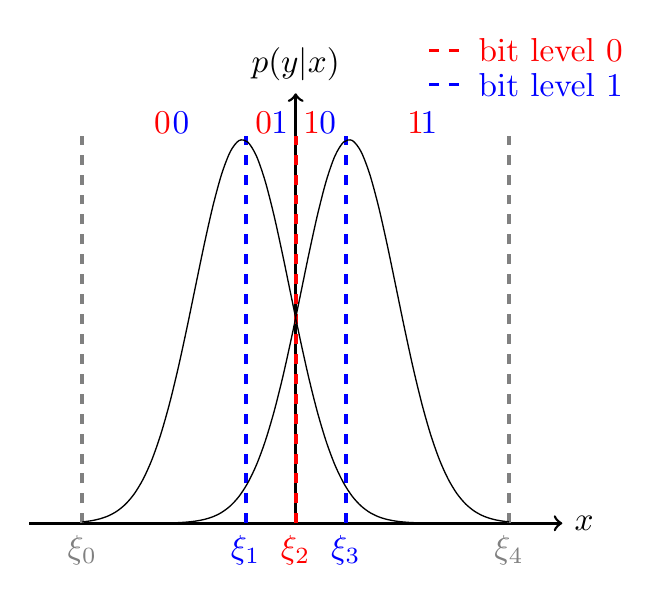
\begin{tikzpicture}[scale = 1.2]
    \begin{axis}[every axis plot post/.append style={
      mark=none,domain=-4:4,samples=50,smooth},
    clip=false,
    axis y line=none,
    axis x line*=bottom,
    ymin=0,
    xtick=\empty,
    ]
    %\draw[help lines, color=gray!30, dashed] (-4.9,0) grid (4.9,0.5);
    \draw[->, thick] (-5,0)--(5,0) node[right]{$x$};
    \draw[->, thick] (0,0)--(0,0.5) node[above]{$p(y|x)$};
    \draw[very thick, dashed, color = red] (0,0)--(0,0.45);
    \node [below, color = red] at (0,0) {{$\xi_2$}};
    \draw[very thick, dashed, color = blue] (0.9400,0)--(0.9400,0.45);
    \node [below, color = blue] at (0.9400,0) {{$\xi_3$}};
    \draw[very thick, dashed, color = blue] (-0.9400,0)--(-0.9400,0.45);
    \node [below, color = blue] at (-0.9400,0) {{$\xi_1$}};
    \draw[very thick, dashed, color = gray] (4,0)--(4,0.45);
    \node [below, color = gray] at (4,0) {{$\xi_4$}};
    \draw[very thick, dashed, color = gray] (-4,0)--(-4,0.45);
    \node [below, color = gray] at (-4,0) {{$\xi_0$}};
    \addplot [color=black] {\gauss{1}{0.8944}};
    \addplot [color=black] {\gauss{-1}{0.8944}};
    \draw[ thick, dashed, color = red ] (2.5,0.55)--(3.2,0.55) node[right]{bit level 0};
    \draw[ thick, dashed, color = blue ] (2.5,0.51)--(3.2,0.51) node[right]{bit level 1};
    \node [above, color = red] at (-2.5,0.44) {0};
    \node [above, color = blue] at (-2.15,0.44) {0};
    \node [above, color = red] at (-0.6,0.44) {0};
    \node [above, color = blue] at (-0.30,0.44) {1};
    
    
    \node [above, color = blue] at (2.5,0.44) {1};
    \node [above, color = red] at (2.25,0.44) {1};
    \node [above, color = blue] at (0.6,0.44) {0};
    \node [above, color = red] at (0.30,0.44) {1};
    
    \end{axis}
    \end{tikzpicture}
	\caption{Given the conditional probability $p(y|x)$ of symmetric BI-AWGN channel, HDQ sequentially quantizing A/D output $w$ into a 2-bit message by first finding the index $\xi_2$, then the indices $\xi_1$ and $\xi_3$.}
	\label{fig: HDQ}
\end{figure}

HDQ quantizes the symmetric BI-AWGN channel output using a  progressive \cite{nathan-hdq} or greedy approach.  
The general $b$-bit HDQ approach is as follows:
\begin{enumerate}
    \item We assume an initial high-precision uniform quantizer.  For this case, set the extreme index thresholds  $\xi_0=0$ and $\xi_{2^b}=B-1$, which are the minimum and maximum outputs of the uniform quantization.  
    \item The index threshold $\xi_{2^{(b-1)}}$ is selected as follows to determine the bit level 0:
    \begin {align}
    \xi_{2^{(b-1)}} = \arg \max_{\xi_0<\xi<\xi_{2^b}} I(X;D_1)\, , 
    \end{align}
where 
\begin{equation} 
D_1 = \mathbbm{1}(W\geq \xi_2^{(b-1)}).
% D_1 = \begin{cases} 
% 0, & \text{if } W < \xi_{2^{(b-1)}}\\
% 1, & \text{otherwise}
%\end{cases}.
\end{equation}

\item The index thresholds  $\xi_{2^{(b-2)}}$ and $\xi_{3*2^{(b-2)}}$ are selected as follows to determine bit level 1:
    \begin {align}
    \xi_{2^{(b-2)}} &= \arg \max_{\xi_0<\xi<\xi_{2^{b-1}}} I(X;D_2| D_1=0), \\ 
    \xi_{3*2^{(b-2)}} &= \arg \max_{\xi_{2^{b-1}}<\xi<\xi_{2^b}} I(X;D_2| D_1=1)\, ,
    \end{align}
    and 
\begin{equation} 
D_2 = \begin{cases} 
\mathbbm{1}(W \geq \xi_{2^{(b-2)}}) & \text{if } D_1=0 \\
\mathbbm{1}(W \geq \xi_{3*2^{(b-2)}}) & \text{if } D_1=1 \\
\end{cases}.
\end{equation}

\item In the general case, when the thresholds for $k$ previous quantization bits have been determined, $2^k$ thresholds $\{\xi_{(j+0.5)2^{b-k}}, j=0,..,2^{k}-1\}$ must be selected to determine the next quantization bit.  Each threshold maximizes $I(X;D_{k+1}|D_k=d_k, \ldots,D_1=d_1 )$ for a specific result for the $k$ previous quantization bits. 
\end{enumerate}


\begin{algorithm}[t]
    \label{alg: HDQ}
    \SetKwInOut{Input}{input}\SetKwInOut{Output}{output}\SetKwProg{Init}{initialization:}{}{}
    
    \Input{$P\left(X,W\right), X\in\{0,1\}, W\in\{0,...,B-1\}$; $b$}
    \Output{ $\{\xi_0,\xi_1,...,\xi_{2^b-1}\}$, $P(X,T)$}
    $\xi_0\leftarrow 0$, 
    $\xi_{2^b}\leftarrow B-1$\\
    \For{$i\gets0$ \KwTo $b-1$ }{
        \For{$j\gets0$ \KwTo $2^{i}-1$ }{
        $\xi_{(j+0.5)2^{b-i}} = \texttt{GSS}(\xi_{j2^{b-i}},\xi_{(j+1)2^{b-i}})$
        }
        }
    $P_{XT}(x,t)=\sum_{w=\xi_t}^{\xi_t+1}P_{XW}(x,w)$, $X\in\{0,1\}$, $T\in\{0,...,2^{b-1}\}$
    \caption{Hierarchical Dynamic Quantization }
    \end{algorithm}
Fig. \ref{fig: HDQ} illustrates how HDQ quantizes the symmetric binary input AWGN for the case where $b=2$. First, the indices  $\xi_0$  and $\xi_4$ of the extreme points are set.  Then the index $\xi_2$ is set to maximize $I(X;D_1)$.  Finally, the indices $\xi_1$ and $\xi_3$ are set to maximize $I(X;D_2| D_1)$ by independently selecting $\xi_1$ to maximize $I(X;D_2| D_1=0)$ and $\xi_3$ to maximize $I(X;D_2| D_1=1)$.


Alg. \ref{alg: HDQ} provides a full description of HDQ algorithm. The function \texttt{GSS}$(\xi_{\ell},\xi_r)$ uses the golden section search algorithm described in Sec.\ref{Sec: GSS} for thresholds search.

HDQ provides the $2^b -1$ index thresholds $\{\xi_1, \ldots, \xi_{2^b-1} \}$. For channel quantization, the index thresholds can be mapped to channel outputs. For the RCQ decoding, the messages are LLR values, the LLR magnitude thresholds $\{\tau_0,\ldots,\tau_{2^{b-1}-2}\}$ are calculated from the index thresholds $\{\xi_{2^{b-1}+1}, \ldots ,\xi_{2^b-1} \}$ as follows:
\begin{align}
\tau_i =~ \log\frac{P_{W|X}(\xi_{1+i+2^{b-1}}|0)}{P_{W|X}(\xi_{1+i+2^{b-1}}|1)}, i=0,1,\ldots,2^{b-1}-2.
\end{align}

HDQ also provides the joint probability between code bit $X$ and quantized message $D$, $P(X,D)$. The magnitude reconstruction function  $R^*(\cdot)$ is computed as follows: 
%to produce LLR magnitudes from quantized messages 
\begin{align}
    R^*(d) = \log\frac{P_{XT}(0,d+2^{b-1})}{P_{XT}(1,d+2^{b-1})},~d=0,1,...,2^{b-1}-1.
    \label{equ: recon_hdq}
\end{align}


\begin{figure}[t]
	\centering
	\includegraphics[width=14pc]{figures/gss.eps}
	\caption{ Illustration of one iteration of golden-section search for finding maximum point of $f(x)$ in the interval $[a_\text{l},a_\text{r}]$. $a'=a_{\text{r}}-\frac{a_\text{r}-a_\text{l}}{\gamma}$ and $a''=a_{\text{l}}+\frac{a_\text{r}-a_\text{l}}{\gamma}$. Because $f(a'')<f(a')$, $[a'',a_\text{r}]$ is truncated and $[a_\text{l},a'']$ becomes the new search interval for the next iteration. 
	}
	\label{fig: gss}
\end{figure}

\subsection{Golden-Section Search and Complexity Analysis}\label{Sec: GSS}
After $k$ stages of HDQ, there are $2^k$ quantization regions each specified by their leftmost and rightmost indices $\xi_{\ell}$ and $\xi_r$.  The next stage finds a new threshold $\xi^*$ for each of these $2^k$ regions.   Each $\xi^*$ is selected to maximize a conditional mutual information as follows:
    \begin{equation}
    \xi^* = \arg \max_{\xi_{\ell}<\xi<\xi_r}  I(\xi),
    \label{equ: optimzation}
    \end{equation}
where 
\begin{align}
      I(\xi) &= I\left(X;D_{k+1}(\xi)|D_1=d_1, \ldots,D_k=d_k \right)\label{equ: I_xi} \\
    &= \sum_{x,d_{k+1}} P\left(x,d_{k+1}(\xi)|d_1^k\right) \log  \frac{P(d_{k+1}(\xi)|x,d_1^k) }{P(d_{k+1}(\xi)|d_1^k) }
\end{align}
for the binary $k$-tuple $d_1^k=d_1, \ldots, d_k$  that defines $(\xi_{\ell}, \xi_r)$. The probability $P\left(x,d_{k+1}(\xi)|d_1^k\right)$ is defined as follows:

\begin{equation}
    P\left(x,d_{k+1}(\xi)|d_1^k\right) = 
    \begin{cases}
    \frac{\sum_{w=\xi_l}^{\xi} P_{XW}(x,w)}{\sum_{w=\xi_l}^{\xi_r} P_{W}(w)} & d_{k+1}=0\\
    \frac{\sum_{w=\xi+1}^{\xi_r} P_{XW}(x,w)}{\sum_{w=\xi_l}^{\xi_r} P_{W}(w)} & d_{k+1}=1\\
    \end{cases}.
\end{equation}

Because $I(\xi)$ is concave in $\xi$, the local maximum can be found using the golden section search \cite{Kiefer1953-pc}, a simple but robust technique to find extreme point of a unimodal function by successively narrowing the range of values on a specified interval. Specifically, Fig. \ref{fig: gss} illustrates one iteration of golden-section search for finding maximum point of $f(x)$ in the interval $[a_\text{l},a_{\text{r}}]$. First, find $a'=a_{\text{r}}-\frac{a_\text{r}-a_\text{l}}{\gamma}$ and $a''=a_{\text{l}}+\frac{a_\text{r}-a_\text{l}}{\gamma}$, where $\gamma = \frac{\sqrt{5}+1}{2}$. Because $f(a'')<f(a')$, which suggests that the maximum point lies in $[a_\text{l},a'']$, the interval $[a'',a_\text{r}]$ is truncated and  $[a_\text{l},a'']$ is updated as the next round search interval. Further details of golden-section search can be found in \cite{Kiefer1953-pc}. When using the golden-section search to find all $2^b -1$ thresholds for the $b$-bit HDQ, $I(\xi)$ will be computed using \eqref{equ: I_xi} a number of times that is proportional to: 
\begin{align}
    &\log_{\gamma}(B)+\sum_{i=1}^{2^1}\log_{\gamma}(B_{2,i})+\ldots+\sum_{i=1}^{2^{b-1}}\log_{\gamma}(B_{b,i}),\\
   =&\log_{\gamma}(B)+\log_{\gamma}\prod_{i=1}^{2^1}B_{2,i}+\ldots+\log_{\gamma}\prod_{i=1}^{2^{b-1}}B_{b,i},\\
    \leq&\log_{\gamma}(B)+2\log_{\gamma}\left(\frac{B}{2}\right)+\ldots+2^{b-1}\log_{\gamma}\left(\frac{B}{2^{b-1}}\right)\\=& \frac{2^b}{\log(\gamma)}\log(B).
\end{align}

$B_{j,i}$ is the $i^{th}$ interval length in ${j-1}$ bit level quantization and $\sum_{i=1}^{2^{j-1}}B_{j,i}=B$. Therefore, a $b$-bit quantization on a  $B$-output channel using HDQ can be designed in $\mathcal{O}\left(\frac{2^b}{\log(\gamma)}\log(B)\right)$ time.

\begin{figure}
	\centering
	\includegraphics[width=18pc]{figures/trellis.eps}
	\caption{A trellis whose paths represent all 2-bit quantizers for a BI-DMC with 8 outputs. The vertices in column $i$ are possible values for $i^{th}$ threshold $\xi_i$. Each branch in the trellis identifies a quantization region.
	}
	\label{fig: trellis}
\end{figure}
\subsection{Comparing HDQ with Optimal Dynamic Programming}
Unlike the dynamic programming approach of Kuskoski and Yagi \cite{Kurkoski2014-QuanDMC}, HDQ does not always provide the optimal solution.  
This subsection provides an example contrasting HDQ with the dynamic programming solution. 
Following \cite{Kurkoski2014-QuanDMC}, Fig. \ref{fig: trellis} gives a trellis whose paths represent all 2-bit quantizers for a binary input DMC with 8 outputs. The outputs are indexed from 0 to 7 and satisfy \eqref{equ: inq}. The vertices in column $i$ are possible values for $\xi_i$, and each path represents a valid quantizer whose thresholds are determined by the vertices in each column. Each branch in the trellis identifies a quantization region. For example, the branch connecting vertex $\xi_0=0$ to vertex $\xi_1=2$ specifies the leftmost quantization region as \{0,1\}, i.e., $\xi_{\ell} = 0$ and $\xi_r =1$.
\begin{figure}[t] 
    \centering
  \subfloat[\label{fig: quan_result}]{%
       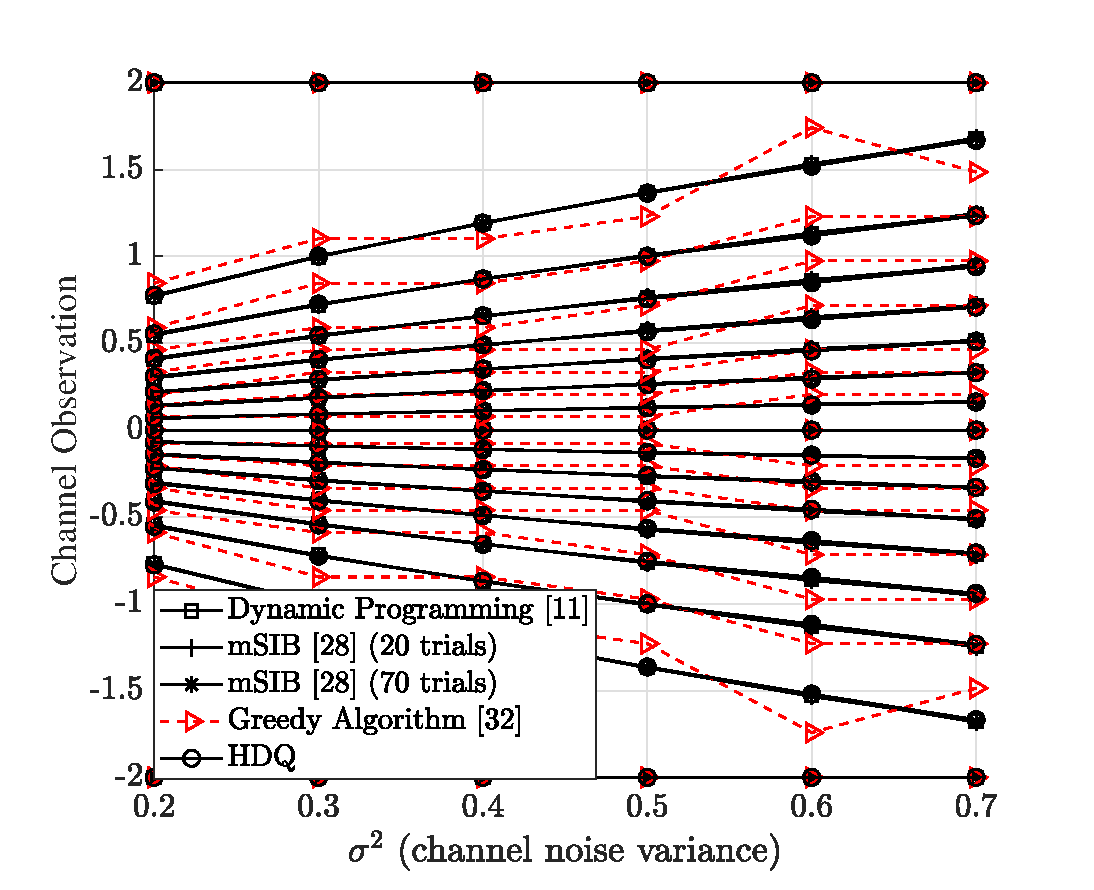
\includegraphics[width=0.5\linewidth]{figures/quantization_result.eps}}
    \hfill
  \subfloat[\label{fig: mi_loss}]{%
        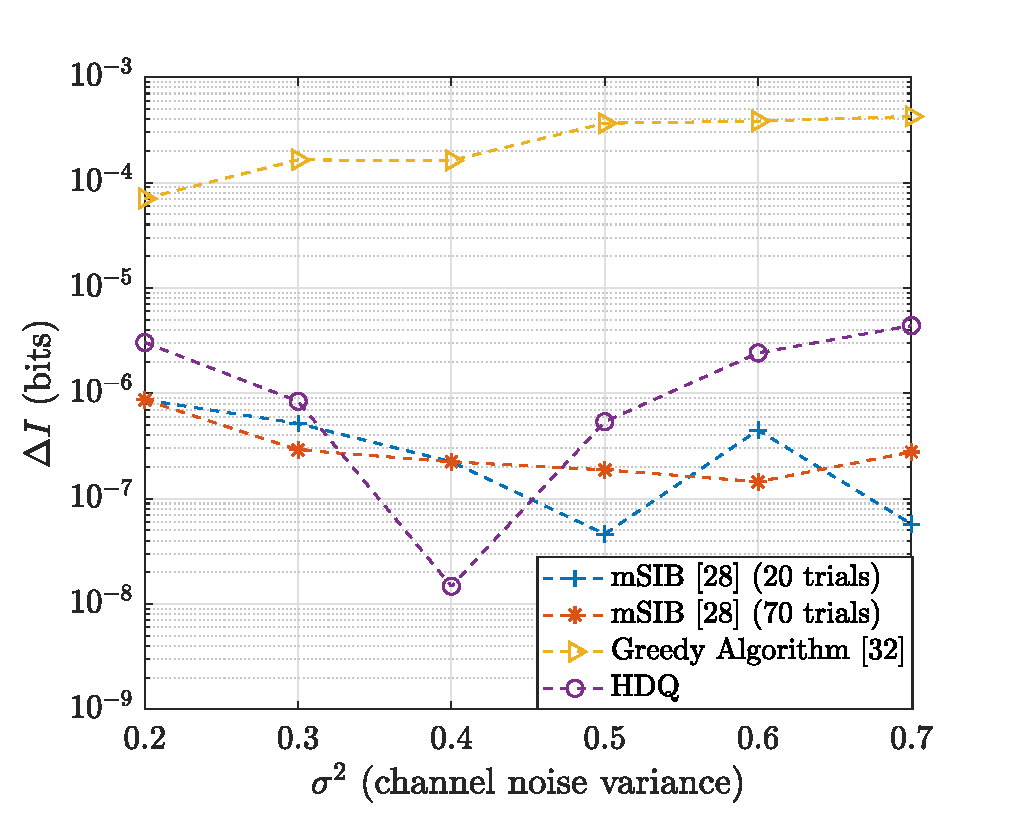
\includegraphics[width=0.5\linewidth]{figures/mutual_info_loss.eps}}
  \caption{Fig. (a): Quantization thresholds for dynamic programming, msIB, and HDQ on the BI-AWGNC as a function of $\sigma^2$ for $B=2000$. Fig. (b): Mutual information loss between each sub-optimal quantizer and optimal quantizer for BI-AWGNC as a function of $\sigma^2$ for $B=2000$. }
\end{figure}

%  Kurkoski's dynamic programming algorithm searches whole trellis and finds the optimal path that maximizes $I(X;D_1,D_2)$. 
The dynamic programming algorithm determines vertices of all columns jointly, whereas HDQ identifies the vertices in a greedy way, by first finding the vertex in column 2 to maximize $I(X;D_1)$ and then vertices in column 1 and 4 to maximize $I(X;D_2|D_1=d_1)$.  Hence, the greedy approach of HDQ only searches part of trellis and therefore is sub-optimal. However, our simulations show that HDQ finds the quantizer that perform closely to  the optimal one.




\subsection{Simulation Result}
This section provides simulation results for quantizing symmetric binary input AWGN channel observations. The simulations compare HDQ to the optimal dynamic programming result as well as to two sub-optimal approaches: mSIB with 20 and 70 trials and the greedy quantization algorithm describe in \cite{Lewandowsky2018-IBRegular}. For all the quantization approaches, the channel observations are first quantized uniformly into $B=2000$ points between $-2$ and $2$. 

Fig. \ref{fig: quan_result} gives the thresholds as a function of $\sigma^2$ for HDQ, dynamic programming, mSIB with 20 and 70 trials, and  greedy quantization.  The quantization thresholds for HDQ, dynamic programming, and mSIB are indistinguishable in Fig.  \ref{fig: quan_result}.  HDQ has significantly lower complexity than both dynamic programming and mSIB. The thresholds for greedy quantization algorithm of \cite{Tal2011-QuanVardy} deviate noticeably from the thresholds found by the other approaches.


In order to quantify the performance of sub-optimal quantizers, we define $\Delta I$ as follows:
\begin{align}
    \Delta I = I^{\text{dp}}(X;D)-I^{\text{sub}}(X;D),
\end{align}
where $I^{\text{dp}}(X;D)$ and $I^{\text{sub}}(X;D)$ are the mutual information between code bit $X$ and quantized value $D$ as obtained by dynamic programming and sub-optimal quantizers, respectively. Fig. \ref{fig: mi_loss} plots $\Delta I$ as a function of $\sigma^2$ for each sub-optimal quantizer.  All three sub-optimal quantizers perform quite well with $\Delta I < 10^{-3}$ bits.  However, HDQ and mSIB achieve  $\Delta I < 10^{-6}$, significantly outperforming the greedy approach of \cite{Tal2011-QuanVardy}.

\section{Flooding-scheduled RCQ Decoder}\label{sec: MIM-DDE}
RCQ decoder is a result of quantized density evolution: In the $t^{th}$ iteration, the quantization functions and the reconstruction functions associated with that iteration, i.e., $Q^c_{t}$, $R^v_t$, $Q^v_t$, $R^v_{t+1}$ are constructed by quantizing the joint p.m.f. between code bits and the message from either the variable node or check node. These functions are also the parameters of the flooding-scheduled RCQ decoder.  To differentiate our discrete density evolution from the one using uniform quantization\cite{Sae-Young_Chung2001-DDE0045}, we name our density evolution \textit{HDQ Discrete Density Evolution} (HDQ-DDE).  Specifically, this section describes the HDQ-DDE when the check node uses box-plus operation. The decoder generated by such HDQ-DDE is a flooding-scheduled bpRCQ decoder.

\subsection{MIM-DDE at check node}
Denote the joint p.m.f between the \textit{external message} from the $i^{th}$ variable node and corresponding code bit  by $P^{v,i}(X,T)$, $X=\{0,1\}$, $T=\{0,\ldots,2^m-1\}$. Based on the independence assumption in density evolution \cite{Richardson2001-de}, all incoming messages have same distribution:
\begin{align}
    P^{v,i} (X,T)=P^v(X,T),\quad i=0,...,d_c-2
\end{align}
where $d_c$ is check node degree. At check node, the code bit corresponding to output is the XOR sum of code bits corresponding to all inputs. By denoting:
\begin{align}
    P^{v,a}(X,T)\circledast P^{v,b}(X,T)\triangleq\sum_{\substack{m,n:\\m\bigoplus n=k} }P^{v,a}(X_m,T)P^{v,b}(X_n,T),
\end{align}
where $m,n,k\in\{0,1\}$, the joint p.m.f between code bit corresponding to output and input messages, $P^c_{out}(X,\mathbf{T})$, can be represented by:
\begin{align}
    P^c_{out}(X,\mathbf{T})&=P^{v,0}(X,T)\circledast ...\circledast P^{v,d_c-2}(X,T)\\
    &=P^{v}(X,T)\circledast ...\circledast P^{v}(X,T)\\
    &\triangleq P^v(X,T)^{\circledast(d_c-1)}, \label{equ: check_opt_prob}
\end{align}
where $\mathbf{T}$ is a vector containing all incoming $d_c-1$ messages.

In order to keep the cardinality of external message the same, $P^c_{out}(X,\mathbf{T})$ needs to be quantized to $2^m$ levels. As pointed in \cite{Lewandowsky2018-IBRegular}, $|\mathbf{T}|=2^{m(d_c-1)}$ will be very large when $m$ and $d_c$ is large. For an example, if $d_c=8$ and $m=4$, $|\mathbf{T}|=2.68*10^8$. Hence, directly quantizing $P^c_{out}(X,\mathbf{T})$ is impossible. To mitigate the problem of \textit{cardinality bombing}, we propose an intermediate coarse quantization algorithm called One-Step-Annealing (OSA) quantization without sacrificing mutual information. Note that Eq. (\ref{equ: check_opt_prob}) can be calculated in a recursive way and each step takes two inputs:
\begin{align}
\label{equ: check_recur}
    P_{out}^{c}(X,\mathbf{T})^{\circledast i}=P^v(X,T)^{\circledast (i-1)}\circledast P^v(X,T) 
\end{align}
We observe that, in each step, the output of Eq.(\ref{equ: check_recur}) has some entries with very close log likelihood ratio (LLR) values. By merging entries whose LLR difference is small enough, mutual information loss is negligible.  Hence, OSA simply merges entries whose LLR values difference is less than a threshold $l_s$, and the output of OSA will be the input of the next p.m.f calculation step, i.e.:
\begin{align}
\label{equ: check_osa}
    P^{v}(X,T)^{\circledast i}= \texttt{OSA}(P^v(X,T)^{\circledast (i-1)},l_s)\circledast P^v(X,T).
\end{align}
\begin{algorithm}[t]
    \label{alg: OSA}
    \SetKwInOut{Input}{input}\SetKwInOut{Output}{output}\SetKwProg{Init}{initialization:}{}{}
    
    \Input{$\Pr\left(X,Y\right), X\in\{0,1\}, Y\in\{0,...,N-1\}$; $l_s$}
    \Output{$\Pr(X,T)$}
    $j\leftarrow0$, 
    $\Pr(X_0,T_j)\leftarrow P(X_0,Y_0)$,
    $\Pr(X_1,T_j)\leftarrow P(X_1,Y_0)$, 
    $l\leftarrow  \log\frac{\Pr(X_0,Y_0)}{\Pr(X_1,Y_0)}$
    
    \For{$i\gets1$ \KwTo $N-1$ }{
          \eIf{$(\log\frac{P(X_0,T_i)}{P(X_1,T_i)}-l)\leq l_s$}
        {
        $P(X_0,T_j)\leftarrow\Pr(X_0,T_j)+\Pr(X_0,Y_i)$, 
        $P(X_1,T_j)\leftarrow\Pr(X_1,T_j)+\Pr(X_1,Y_i)$
        }
        {
        $j\leftarrow j+1$\\
        $\Pr(X_0,T_j)\leftarrow\Pr(X_0,Y_i)$, $\Pr(X_1,T_j)\leftarrow\Pr(X_1,Y_i)$\\
        $l\leftarrow\log\frac{\Pr(X_0,Y_i)}{\Pr(X_1,Y_i)}$
        }
        }
    \caption{One Step Annealing Algorithm (OSA) }\label{sec: MIMDDE}
\end{algorithm}
\begin{figure}
	\centering
	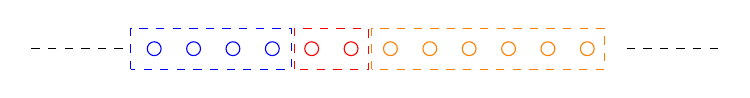
\begin{tikzpicture}[scale = 2.0]


\node[circle,draw=blue, fill=white, inner sep=0pt,minimum size=5pt] (b) at (-1,0) {};
\node[circle,draw=blue, fill=white, inner sep=0pt,minimum size=5pt] (b) at (-0.25,0) {};
\node[circle,draw=blue, fill=white, inner sep=0pt,minimum size=5pt] (b) at (-0.5,0) {};
\node[circle,draw=blue, fill=white, inner sep=0pt,minimum size=5pt] (b) at (-0.75,0) {};
\node[circle,draw=red, fill=white, inner sep=0pt,minimum size=5pt] (b) at (0,0) {};
\node[circle,draw=red, fill=white, inner sep=0pt,minimum size=5pt] (b) at (0.25,0) {};
\node[circle,draw=orange, fill=white, inner sep=0pt,minimum size=5pt] (b) at (0.5,0) {};
\node[circle,draw=orange, fill=white, inner sep=0pt,minimum size=5pt] (b) at (0.75,0) {};
\node[circle,draw=orange, fill=white, inner sep=0pt,minimum size=5pt] (b) at (1,0) {};
\node[circle,draw=orange, fill=white, inner sep=0pt,minimum size=5pt] (b) at (1.25,0) {};
\node[circle,draw=orange, fill=white, inner sep=0pt,minimum size=5pt] (b) at (1.5,0) {};
\node[circle,draw=orange, fill=white, inner sep=0pt,minimum size=5pt] (b) at (1.75,0) {};
\draw[black, dashed] (2.0,0)--(2.6,0);
\draw[black, dashed] (-1.2,0)--(-1.8,0);
\draw [blue, dashed] (-1.15,-0.13) rectangle (-0.13,0.13);
\draw [red, dashed] (-0.11,-0.13) rectangle (0.36,0.13);
\draw [orange, dashed] (0.38,-0.13) rectangle (1.86,0.13);
\end{tikzpicture}
	\caption{OSA illustration: points are ordered w.r.t. LLR values. Each color represents a cluster and LLR value difference in each cluster is less than $l_s$. }
	\label{fig: OSA}
\end{figure}


    

We use $l_s\in[10^{-4},10^{-3}]$ in our simulation. Fig. \ref{fig: OSA} shows an illustration of OSA and a full description of the OSA algorithm is given in Algorithm.\ref{alg: OSA}. The following table shows $|\mathbf{T}|$ after we implement OSA and choose different $l_s$. The example we show has the parameter $m=4$, $d_c=8$. The result shows that OSA greatly decreases the output cardinality, and based on our simulation, mutual information losses under these three $l_s$ are all less than $10^{-7}$ bits.
\begin{table}[hp]
\centering
\begin{tabular}{|c|c|c|c|c|}
\hline
$l_s$                                                         & $0$           & $10^{-4}$    & $5*10^{-4}$ & $10^{-3}$  \\ \hline
\begin{tabular}[c]{@{}c@{}}$|\mathbf{T}|$\end{tabular} & $2.68*10^{8}$ & $3.3*10^4$ & $1.7*10^3$  & $1.3*10^3$ \\ \hline
\end{tabular}
\end{table}

\subsection{MIM-DDE at variable node}

Each variable node sums the LLR messages from its channel observation and neighboring check nodes. By denoting: 

\begin{align}
P^{c,a}(X,T)\boxdot P^{c,b}(X,T)&=\frac{1}{P(X)}P^{c,a}(X,T)P^{c,b}(X,T),
\end{align}
the joint p.m.f between code bit $X$ and incoming message combination $\mathbf{T}$, $P^v_{out}(X,\mathbf{T})$, given variable node degree $d_v$,  can be expressed by:
\begin{align}
    P^v_{out}(X,\mathbf{T})=P^{ch}(X,T)\boxdot P^c(X,T)^{\boxdot(d_v-1)},
\end{align}
Similarly, for irregular LDPC codes with variable edge degree distribution $\lambda(x)=\sum_{i=2}^{d_{v,max}}\lambda_ix^{i-1}$, $P^v_{out}(X,\mathbf{T})$ is given by:
\begin{align}
     P^v_{out}(X,\mathbf{T})=P^{ch}(X,T)\boxdot \sum_{i=2}^{d_{v,max}}\lambda_i P^c(X,T)^{\boxdot(d_v-1)}.
\end{align}
$P_{out}^v(X,\mathbf{T})$ is then quantized to $2^m$ levels by HDQ. Also, as a result of HDQ, and joint p.m.f between code bit $X$ and quantized messages $T$, $P^v(X,T)$, is updated. $Q^v$ in this iteration and $R^c$ in the next iteration are built correspondingly. Note that variable nodes also face the \textit{cardinality bombing} problem, hence $\texttt{OSA}$ is needed in each  recursive step. 



Thus, by implementing MIM-DDE, we can iteratively update $P^c(X,T)$, $P^v(X,T)$ and build $Q^c_i$, $Q^v_i$, $R^c_i$ and $R^v_i$, $i=\{0,...,I_T-1\}$. 

In MIM-DDE, we only limit the precision of external messages, i.e. $m$, and keep internal messages, $n^c$ (only for \textit{bp-RCQ}) and $n^v$, full precision. To make internal message precision finite, a uniform $n^c$ (or $n^v$) quantizer is required when implementing ${F}^c$(or ${F}^v$).

\subsection{Threshold}
At any specified $\frac{E_b}{N_o}$, flooding-scheduled HDQ discrete density evolution constructs the $R^{(t)}(\cdot)$ and $Q^{(t)}(\cdot)$ functions  at each iteration $t$ and also computes the mutual information $I^{(t)}\left(\frac{E_b}{N_o}\right)$ between a code bit and its corresponding variable node message in each layer $r$ at each iteration $t$. An important design question is which value of $\frac{E_b}{N_o}$ to use to construct the $R^{(t)}(\cdot)$ and $Q^{(t)}(\cdot)$ functions implemented at the decoder, which necessarily will work over a range of $\frac{E_b}{N_o}$ values in practice.  Define the threshold of a flooding RCQ decoder given a maximum number of decoding iterations $I_T$ as: 
\begin{align}
    \frac{E_b}{N_o}^*=\inf \left\{\frac{E_b}{N_o}:  I^{(I_T)}\left(\frac{E_b}{N_o}\right)> 1-\epsilon\right\},
\end{align}
i.e., $\frac{E_b}{N_o}^*$ is the smallest $\frac{E_b}{N_o}$ that achieves a mutual information between the  code bit and the external message that is greater that $1-\epsilon$. Our simulation results show that  $\frac{E_b}{N_o}^*$ for $\epsilon = 10^{-4}$ produced $R^{(t)}(\cdot)$ and $Q^{(t)}(\cdot)$ functions that deliver excellent FER performance across a wide $\frac{E_b}{N_o}$ range. 

\section{Layered-scheduled RCQ Decoder}\label{sec: layered}

 This section is focused on HDQ discrete density evolution for LDPC decoders with a  layered schedule. Specifically, this section considers layer-specific msRCQ decoding on QC-LDPC codes.


\subsection{Decoding a Quasi-Cyclic LDPC Code with a Layered Schedule}\label{sec: QC_layer}

QC-LDPC codes are structured LDPC codes characterized by a parity check matrix $H\in \mathbb{F}_2^{(n-k)\times n}$ which consists of square sub-matrices with size $S$, which are either the all-zeros matrix or a cyclic permutation of the identity matrix.   These cyclic permutations  are also called circulants that are represented by $\sigma^i$ to indicate that the rows of the identity matrix are  cyclically shifted  by $i$ positions.  Thus an $M\times U$ \emph{base matrix} $H_\text{p}$ can concisely define a QC-LDPC code, where each element in $H_\text{p}$ is either $\mathbf{0}$ (the all-zeros matrix) or $\sigma^i$ (a circulant). QC-LDPC codes are  perfectly compatible with horizontal layered decoding by partitioning CNs into $M$ layers with each layer containing $S$ consecutive rows. This ensures that each VN connects to at most one CN in each layer.

Denote the $i^{th}$ CN and $j^{th}$ VN by $c_i$ and $v_j$ respectively. Let $u^{(t)}_{c_i\rightarrow v_j}$ be the LLR message from $c_i$ to its neighbor $v_j$ in $t^{th}$ iteration and $l_{v_j}$ be the posterior of $v_j$.  In the $t^{th}$ iteration, a  horizontal-layered \minsum decoder calculates the messages $u^{(t)}_{c_i\rightarrow v_{j'}}$ and updates the posteriors $l_{v_{j'}}$ as follows:
\begin{align}
    {l}_{v_{j'}} &\leftarrow  l_{v_{j'}}- u^{(t-1)}_{c_i\rightarrow v_{j'}}~~\forall j'\in\mathcal{N}(c_i),\label{equ: v-c}
\end{align}
\begin{align}
        u^{(t)}_{c_i\rightarrow v_{j'}} &=
    \left(\prod_{\tilde{j}\in\mathcal{N}(c_i)/\{{j'}\}}\text{sign}(l_{v_{\tilde{j}}})\right)\times\min_{\tilde{j}\in\mathcal{N}(c_i)/\{{j'}\}}|l_{v_{\tilde{j}}}|,~~\forall j'\in\mathcal{N}(c_i), \label{equ: c-v}
\end{align}
\begin{align}
    l_{v_{j'}} &\leftarrow {l}_{v_{j'}}+u^{(t)}_{c_i \rightarrow v_{j'}} ~~\forall j'\in\mathcal{N}(c_i)\label{equ: posteriot_up}.
\end{align}
$\mathcal{N}(c_i)$ denotes the set of VNs that are neighbors of $c_i$.  For a QC-LDPC code with a long block length, layered decoding is preferable for hardware implementations because  parallel computations of each of \eqref{equ: v-c}, \eqref{equ: c-v}, and \eqref{equ: posteriot_up} exploit the QC-LDPC structure. 


\begin{figure}[t] 
    \centering
  \subfloat[ \label{fig: nonlayered_RCQ_str}]{%
      \includegraphics[width=0.5\linewidth]{figures/RCQ_nonlayered.eps}}
\hfill
  \subfloat[\label{fig: layered_RCQ_str}]{%
        \includegraphics[width=0.5\linewidth]{figures/RCQ_layered.eps}}
  \caption{ Two layered decoders. Fig. (a) uses the same RCQ parameters for each layer as with the  \textit{msRCQ} design for a flooding decoding in \cite{Wang2020-RCQ}. Fig. (b) shows the proposed \textit{layer-specific msRCQ} decoder in \cite{Terrill2021-ec}, which features  separate RCQ parameters for each layer.
  The main difference is that msRCQ decoder uses iteration specific parameters while L-msRCQ decoder considers layer-and-iteration parameters.
  }
  \label{fig: gradient_explosion} 
\end{figure}

\subsection{Representation Mismatch Problem}
The RCQ decoding structure in \cite{Wang2020-RCQ} can be used with a layered schedule as discussed in Sec. \ref{sec: QC_layer}. Fig. \ref{fig: nonlayered_RCQ_str} illustrates the paradigm for an msRCQ decoder with a layered schedule. The $Q_\text{v}^{(t)}$ and $R_\text{v}^{(t)}$ are designed by the HDQ discrete density evolution as in \cite{Wang2020-RCQ}. Even though the msRCQ decoder has better FER performance than the standard \minsum decoder under a flooding schedule\cite{Wang2020-RCQ}, under a layered schedule, msRCQ has worse FER performance than standard \minsum and also requires more iterations.  These performance differences are shown below in Fig.  \ref{fig: 8k_performance} of Sec. \ref{sec: simulation result}. This subsection explains how the performance degradation of the RCQ decoder under the layered schedule is caused by the representation mismatch problem. 


Consider a  regular LDPC code defined by a parity check matrix $H$. In iteration $t$, define the PMF between code bit $x$ and external CN messages $u^{(t)}_{c_i \rightarrow v_j}$ as $P^{(t)}_{(c_i,v_j)}(X,D)$, where $X=\{0,1\}$ and $D=\{0,...,2^{b^\mathrm{e}}-1\}$. One underlying assumption of HDQ discrete density evolution is that all CN messages have the same PMF in each iteration, i.e., for any $(c_{i},v_{j})$ and $(c_{i'}, v_{j'})$ that satisfy $H_{i,j}=H_{i',j'}=1$:
\begin{align}
    P^{(t)}_{(c_i,v_j)}(X,D) = P^{(t)}_{(c_{i'},v_{j'})}(X,D).
    \label{equ: Assumption_on_MIM_DDE}
\end{align}
(\ref{equ: Assumption_on_MIM_DDE}) implies that the message indices of different CN have the same LLR representation, i.e.:
\begin{align}
    \log\frac{P^{(t)}_{(c_i,v_j)}(0,d)}{P^{(t)}_{(c_i,v_j)}(1,d)} = \log\frac{P^{(t)}_{(c_{i'},v_{j'})}(0,d)}{P^{(t)}_{(c_{i'},v_{j'})}(1,d)},~   d\in \{0,...,2^{b^\mathrm{e}}-1\}.
    \label{equ: Assumption_on_MIM_DDE2}
\end{align}
 The msRCQ decoder with a flooding schedule obeys (\ref{equ: Assumption_on_MIM_DDE}) and (\ref{equ: Assumption_on_MIM_DDE2})  because the VN messages to calculate different CN messages have the same distribution. Therefore, it is sufficient for a decoder with a flooding schedule  to use the iteration-specific reconstruction function  $R^{(t)}$ for all external CN messages. However, for a decoder with a layered schedule, the VN messages to calculate CN messages from different layers have different distributions. For the decoder with a layered schedule, $l^{(t)}_{v_j\rightarrow c_i}$ is calculated by:
\begin{align}\label{equ: vari_update_2}
    l^{(t)}_{v_j\rightarrow c_i} = l^{(ch)}_{v_j}&+ \sum_{\{i'|{i'}\in\mathcal{N}(v_j),i'<i\}}u^{(t)}_{c_{i'}\rightarrow v_{j}}+ \sum_{\{i'|{i'}\in\mathcal{N}(v_j),i'>i\}}u^{(t-1)}_{c_{i'}\rightarrow v_{j}},
\end{align}
%We omit $R(\cdot)$ in Eq.(\ref{equ: vari_update_2}) by abuse of notation. 
Unlike a decoder using a flooding schedule, which updates $ l^{(t)}_{v_j\rightarrow c_i}$ only using CN messages in iteration $t-1$, decoders using a layered schedule use messages from both iteration $t-1$ and iteration $t$. The VN messages computed in different layers utilize different proportions of check-to-variable node messages from iterations $t-1$ and $t$.  Since the check-to-variable node messages from different iterations have different reliability distributions, the VN messages from different layers also have different distributions. Therefore \eqref{equ: Assumption_on_MIM_DDE} and \eqref{equ: Assumption_on_MIM_DDE2} no longer hold true, and a single $R^{(t)}(\cdot)$ is insufficient to accurately describe CN messages from different layers. 

In conclusion, the \textit{Representation Mismatch Problem} refers to inappropriately using a single $R^{(t)}$ and single $Q^{(t)}$ for all layers in iteration $t$  of a layered decoding schedule. This issue degrades the decoding performance of layer-scheduled RCQ decoder.  On the other hand, the conventional fixed-point decoders that do not perform coarse non-uniform quantization, such as standard \minsum decoder,  are not affected by the changing the distribution of messages in different layers and hence don't have representation mismatch problem.

\subsection{Layer-Specific RCQ Design}
Based on the analysis in the previous subsection,  $R$ and $Q$ should adapt for the PMF of messages in each layer, in order to solve the representation mismatch problem. This motivates us to propose the layer-specific RCQ decoding structure in this paper, as illustrated in Fig. \ref{fig: layered_RCQ_str}. The key difference between the RCQ decoder and layer-specific RCQ decoder is that layer-specific RCQ designs quantizers and reconstruction mappings for each layer in each iteration.  We use $R^{(t,r)}$ and $Q^{(t,r)}$ to denote the reconstruction mapping and quantizer for decoding iteration $t$ and layer $r$, respectively. 
As illustrated in Fig. \ref{fig: layered_RCQ_str}, layer-specific RCQ specifies $R$ and $Q$ for each layer to handle the issue that messages in different layers have different PMFs. This leads to a significant increase in the required memory because the memory required to store $R^{(t,r)}$ and $Q^{(t,r)}$ is proportional to the product of the number of layers and the number of iterations required for decoding the QC-LDPC code.

Designing $Q^{(t,r)}(\cdot)$ and $R^{(t,r)}(\cdot)$ for layer-specific msRCQ requires the message PMF for each layer in each iteration.  However, HDQ discrete density evolution\cite{Wang2020-RCQ}, which performs density evolution based on ensemble, fails to capture layer-specific information. In this section, we propose a layer-specific HDQ discrete density evolution based on base matrix $H_\text{p}$ of QC-LDPC code. In layer-specific HDQ discrete density evolution, the joint PMF between code bit $X$ and external message $D$ from check/variable nodes are tracked in each layer in each iteration. We use $P^{(t,r)}(X,D^\text{c})$, $X\in\{0,1\}$, $D^\text{c}\in\{0,\ldots,2^{b^\text{e}}-1\}$ to represent the joint PMF between code bit and CN message in layer $m$ and iteration $t$. Similarly, VN messages are denoted by $P^{(t,r)}(X,D^\text{v})$.

\subsubsection{Initialization}
For an AWGN channel with noise variance $\sigma^2$, the LLR of channel observation $y$ is $l=\frac{2}{\sigma^2}y$.
For the msRCQ decoder with bit width $(b^\text{e},b^\text{v})$, the continuous channel LLR input is uniformly quantized into $2^{b^\text{v}}$ regions.  Each quantization region has a true log likelihood ratio, which we refer to as $l_d$, so that we have an alphabet of $b^\text{v}$ real-valued log likelihood ratios ${\mathcal D}^{\text{ch}}=\{l_0,...,l_{2^{b^{\text{v}}}-1}\}$.  Using these values, the joint PMF between the code bit $X$ and channel LLR message $D^{\text{ch}} \in \{0,...,{2^{b^{\text{v}}}-1}\}$ is:
\begin{align}\label{equ: chan_prob}
    P_{XD^{\text{ch}}}(x,d) &= P_D(d) \frac{e^{(1-x)l_d}}{e^{l_d}+1}, ~X\in \{0,1\},\  l_d\in {\mathcal D}^{\text{ch}}\, .
\end{align}
The distribution $P_{XD^{\text{ch}}}(x,d)$ is used for the HDQ discrete density evolution design.  The actual decoder does not use the real-valued likelihoods $l_d$ but rather uses $b^{\text{v}}$-bit channel LLRs obtained by uniformly quantizing continuous channel LLR values.
\subsubsection{Variable Nodes PMF Calculation}
Given a base matrix $H_\text{p}$, with entry $H_\text{p}(r,c)$ at row $r$ and column $c$, define the sets of active rows $\mathcal{R}(c)$ for a specified column $c$ and active columns $ \mathcal{C}(r)$ for a specified row $r$ as follows:
\begin{align}
\mathcal{R}(c) = \{r| H_\text{p}(r,c)\neq0\}
,\quad 
\mathcal{C}(r)= \{c| H_\text{p}(r,c)\neq0\}.
\end{align}
In iteration $t$ and layer $r$, consider the joint PMF between a code bit $X$ corresponding to a VN in the circulant $H_\text{p}(r,c)$ and the vector $\mathbf{D}$, which includes the channel message $D^{\text{ch}}$ for $X$ and the check node messages $D^{\text{c}}$ incident to that VN.  This PMF is calculated by:
\begin{align}
\begin{split}
        P_\text{v}^{(t,r,c)}(X,\mathbf{D})&=P(X,D^{\text{ch}})\boxdot\left(\boxdot_{\substack{k\in\mathcal{R}(c) \\ k<r}}P^{(t,k)}(X,D^{\text{c}})\right) \\&\boxdot\left(\boxdot_{\substack{k\in\mathcal{R}(c) \\ k>r}}P^{(t-1,k)}(X,D^{\text{c}})\right), 
\end{split}
    \label{eq: vari_update}
\end{align}
$\boxdot$ is defined as follows: 
\begin{align}
    P(x,[d_1,d_2])&=P({X_1,D_1})\boxdot P({X_2,D_2})\\&\triangleq\frac{1}{P_X(x)}P_{X_1D_1}(x,d_1)P_{X_2D_2}(x,d_2),
\end{align}
% Unlike HDQ-DDE, which takes the same PMF to all incoming messages from different layers ( (12) in \cite{Wang2020-RCQ}), Eq.(\Ref{eq: vari_update}) utilizes layer-specific PMF. 
$ x\in\{0,1\},~d_1,d_2\in\{0,\ldots,2^{b^\mathrm{e}}-1\}$. When $|\mathcal{R}(c)|$ is large, the alphabet ${\mathcal D}$ of possible input message vectors $\mathbf{D}$ is large with $|{\mathcal D}|=2^{b^\mathrm{v}+(|\mathcal{R}(c)|-1)b^\mathrm{e}}$.  To manage the complexity of HDQ discrete density evolution, message vectors $\mathbf{D}$ with similar log likelihoods are clustered via  one-step-annealing as in \cite{Wang2020-RCQ} for (\Ref{eq: vari_update}).

The layer-specific msRCQ decoder uses layer-specific parameters, and for each layer the marginal distribution on the computed variable node messages will be distinct. The marginal distribution used by HDQ at layer $r$ is computed as follows:
\begin{align}\label{eq: vari_total}
    \Tilde{P}_\text{v}^{(t,r)} = \left\{\frac{1}{|\mathcal{C}(r)|}P_\text{v}^{(t,r,c)}(X,\mathbf{D})\mid c\in\mathcal{C}(r)\right\}\,
\end{align}
 where ${P}^{(t,r)}(X,D^v)$ and $Q^{(t,r)}(\cdot)$ can be obtained by quantizing  $\Tilde{P}_\text{v}^{(t,r)}$ using HDQ:
\begin{align}\label{eq: vari_hdq}
    \left[P^{(t,r)}(X,D^{\text{v}}),Q^{(t,r)}(\cdot) \right] = \texttt{HDQ}\left(\Tilde{P}_\text{v}^{(t,r)}, 2^{b^\mathrm{e}}\right),
\end{align}
where \texttt{HDQ} is defined as a function that realizes $b^e$-bit HDQ on  $\Tilde{P}_\text{v}^{(t,r)}$ and generates $P^{(t,r)}(X,D^{\text{v}})$ and $Q^{(t,r)}$ as outputs. Note that (33) and (34) realize implicit message alignment in \cite{Stark2021-ai} such that the internal messages from  any  $c\in\mathcal{C}(r)$  use same set of thresholds for quantization and the same external messages from any $c\in\mathcal{C}(r)$ have same LLR interpretations, regardless of node degree.

\subsubsection{Check Nodes PMF Calculation}
Let $l^{(t,r)}_\text{v}{(d)}$ be the LLR of external VN message $d$ in layer $r$ and iteration $t$.  As an LLR, this CN input  $l^{(t,r)}_\text{v}{(d)}$ has the following meaning: 
\begin{align}
    l_\text{v}^{(t,r)}(d) = \log \frac{P_{XD^\text{v}}^{(t,r)}(0,d)}{P_{XD^\text{v}}^{(t,r)}(1,d)},\quad d=0,...,2^{b^{e}}-1.
\end{align}
Given input messages $d_1,d_2\in {\mathcal D}^\text{v}$, the CN min operation produces the following output:
\begin{align}\label{equ: label_min}
\begin{split}
     l_{\text{MS}}^{\text{out}} =&\min\left(|l_\text{v}^{(t,r)}(d_1)|,|l_\text{v}^{(t,r)}(d_2))|\right)\\&\times \text{sgn}(l_\text{v}^{(t,r)}(d_1))\times\text{sgn}(l_\text{v}^{(t,r)}(d_2)). 
\end{split}
\end{align}
Under the symmetry assumption, there is a $d^{\text{out}}\in {\mathcal D}^\text{v}$ that has the LLR computed as $l_{\text{MS}}^{\text{out}}$:
\begin{align}\label{equ: label_min_2}
    l_{\text{MS}}^{\text{out}}=\log \frac{P^{(t,r)}_{XD^\text{v}}(0,d^{\text{out}})}{P^{(t,r)}_{XD^\text{v}}(1,d^{\text{out}})}.
\end{align}
At the check node output, $l_{MS}^{out}$ will be assigned the label $d^{out}\in {\mathcal D}^v$ that satisfies \eqref{equ: label_min_2}.  However, the LLR meaning associated with that $d^{out}$ must be adjusted. 

Define the follow function: 
\begin{align}\label{equ: label-min}
    d^\text{out} = \texttt{MS}(d_1,d_2),
\end{align}
 where $d^{\text{out}},d_1,d_2\in \mathcal{D}^\mathrm{v} $. \eqref{equ: label-min} holds if and only if \eqref{equ: label_min} and \eqref{equ: label_min_2} and are both satisfied.


Define the binary operation $\circledast$ by:
\begin{align}
          \Tilde{P}_{XD}(x,d) &= P(X_1,D_1)\circledast P(X_2,D_2)\\&\triangleq\sum_{\substack{d_1,d_2:\texttt{MS}(d_1,d_2)=d \\ x_1,x_2: x_1\bigoplus x_2 = x}}P_{X_1D_1}(x_1,d_1)P_{X_2D_2}(x_2,d_2)\label{equ: msrcq-c}.
\end{align}


%To obtain the new LLR for $d^{out}$, 
The joint PMF between code bit and external CN message in layer $r$ and iteration $t$ can be updated by:
\begin{align}
 P^{(t,r)}(X,D^\text{c}) &=P^{(t,r)}(X,D^\text{v})\circledast ...\circledast P^{(t,r)}(X,D^\text{v})\\&\triangleq P^{(t,r)}(X,D^\text{v})^{\circledast(|\mathcal{C}(r)|-1)}. \label{equ: check_opt_prob2}
\end{align}
$R^{(t,r)}(\cdot)$ can be directly computed using $P^{(t,r)}(X,D^\text{c})$:
\begin{align}
        R^{(t,r)}(d) = \log \frac{P_{XD^\text{c}}^{(t,r)}(0,d)}{p_{XD^\text{c}}^{(t,r)}(1,d)},~d\in\{0,...,2^{b^\text{e}}-1\}.
        \label{eq: r_v}
\end{align}

\subsection{Threshold}
The threshold of a layer-specific RCQ decoder given a base matrix with $M$ layers and  maximum number of decoding iterations $I_T$ is defined as: 
\begin{align}
    \frac{E_b}{N_o}^*=\inf \left\{\frac{E_b}{N_o}:  I^{(I_T,r)}\left(\frac{E_b}{N_o}\right)> 1-\epsilon,\forall  r\in[1,M] \right\}.
\end{align}

\begin{figure}[t] 
    \centering
  \subfloat[Decoders with floating point messages\label{fig: 80211_1}]{%
       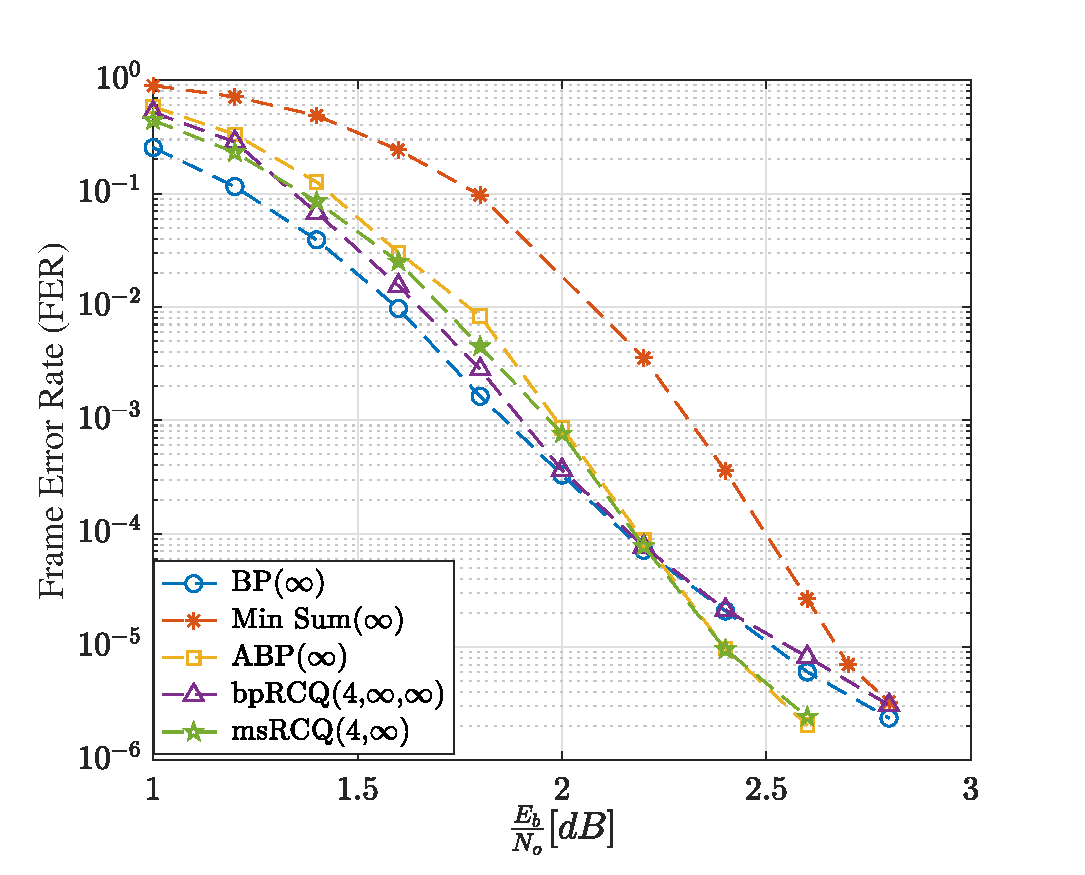
\includegraphics[width=0.5\linewidth]{figures/80211_fig1.eps}}
    \hfill
  \subfloat[Decoders with fixed point messages\label{fig: 80211_3}]{%
        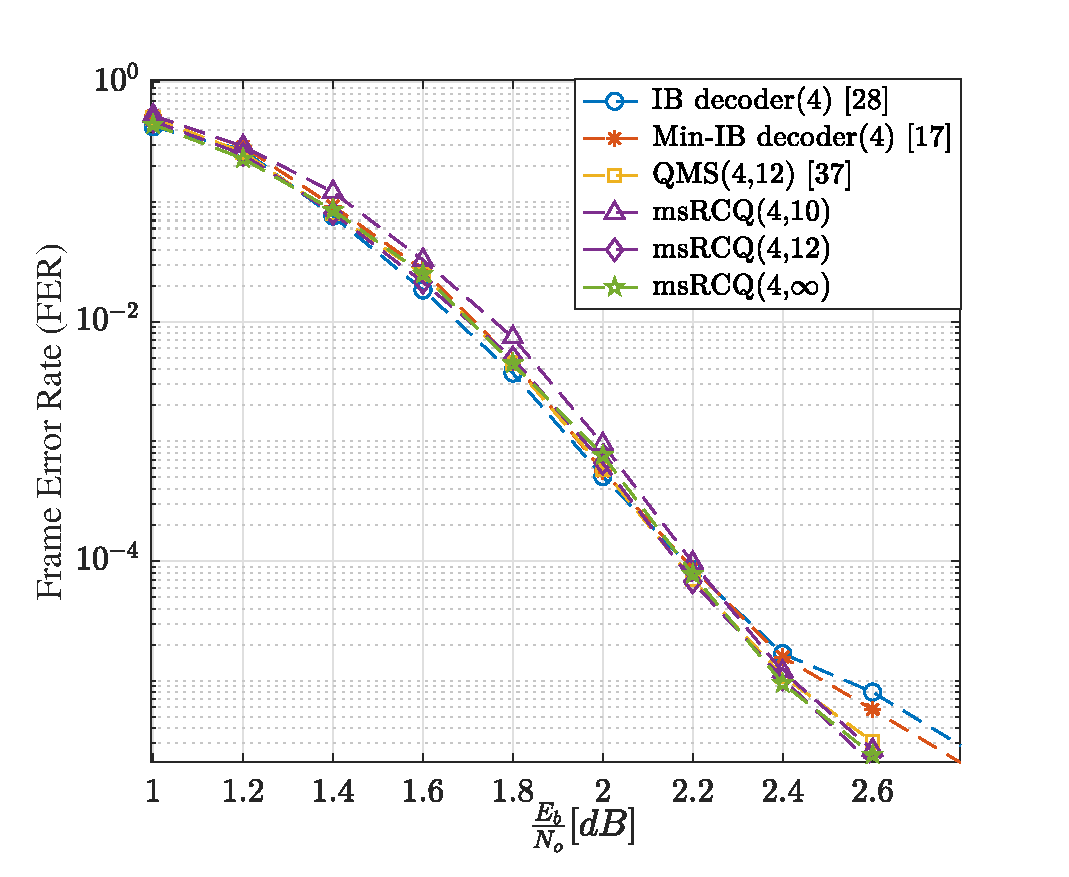
\includegraphics[width=0.5\linewidth]{figures/80211_fig3.eps}}
  \caption{Fig. (a): FER performance of 4-bit msRCQ and bpRCQ decoders with floating point message representations use at the VNs.  Fig. (b):FER performance of fixed point 4-bit msRCQ decoders, compared with other non-uniform quantization decoders. }
\end{figure}

\section{Simulation Result and Discussion}\label{sec: simulation result}
This section presents RCQ and layer-specific RCQ decoder designs for two example LDPC codes and compares their FER performance  with existing conventional decoders such as BP, \minsum, and state-of-the-art non-uniform decoders, such as an IB decoder. All decoders are simulated using the AWGN channel, and at least 100 frame errors are collected for each point.  We also compare hardware requirements for an example LDPC code.
\subsection{IEEE 802.11 Standard LDPC Code}
We first investigate the FER performance of RCQ decoders with a flooding schedule using an IEEE 802.11n standard LDPC code taken from \cite{80211spec}. This code has $n=1296$, $k=648$, and the edge distribution is:
\begin{align}
    \lambda(x) &= 0.2588x+0.3140x^2+0.0465x^3+0.3837x^{10}, \\
    \rho(x) &= 0.8140x^6 +0.1860 x^7.
\end{align}
The maximum number of decoding iterations was set to 50.

Fig. \ref{fig: 80211_1} shows the FER curves of  4-bit bpRCQ and msRCQ decoder with floating-point internal messages, i.e., {bpRCQ}(4,$\infty$,$\infty$) and {msRCQ}(4,$\infty$), respectively . The notation of $\infty$ represents floating-point message representation. Denote floating point BP nad Min Sum by BP($\infty$) and Min Sum($
\infty$), respectively.  The 4-bit bpRCQ decoder has at most 0.1 $dB$ degradation compared with the floating-point BP decoder, and outperforms floating-point BP at high $\frac{E_b}{N_o}$.  The 4-bit msRCQ performs better than conventional \minsum and even surpasses BP at high $\frac{E_b}{N_o}$. The lower error floor of msRCQ decoder as compared to standard BP follows from the slower message magnitude convergence rate as compared to standard BP. This is similar to improved error floors achieved by the averaged BP (ABP) [35], which  decreases the rate of increase of message magnitudes by averaging the posteriors  $l_v^{(t)}$ in consecutive iterations. As shown in Fig. \ref{fig: 80211_1}, ABP also delivers a lower error floor than standard BP.

 The slow magnitude convergence rate of msRCQ decoder can be explained as follows.  For conventional \minsum decoder, the magnitude of each check node message is always equal to the magnitude of an input variable node message for that CN.  This is not true for the msRCQ decoder. msRCQ compares the relative LLR meanings of input messages and returns an external message by implementing the min operation. However, the external message is then reconstructed at the VN to an internal message magnitude that is in general different from the message magnitudes that were received by the neighboring CN. 

 For the example of a degree-3 CN, \eqref{equ: ave_msrcq} computes the likelihood associated with a message $l_t$ that is outputted from the min operation applied to the other two input messages indexed by $i$ and $j$:
\begin{align}\label{equ: ave_msrcq}
    l_{t}&=\log\frac{\sum_{\{(i,j)|t=MS(i,j)\}}P(0,i)P(0,j)+P(1,i)P(1,j)}{\sum_{\{(i,j)|t=MS(i,j)\}}P(1,i)P(0,j)+P(0,i)P(1,j)}. 
\end{align}
Note that the boxplus operation is computed as follows :
\begin{align}
   l_i\boxplus l_j &=\log \frac{P(0,i)P(0,j)+P(1,i)P(1,j)}{P(0,i)P(1,j)+P(1,i)P(0,j)}\label{equ: box_plus_p}.
\end{align}
MinSum is an approximation to the boxplus operation, and boxplus produces a range of message values for edges that would share the same MinSum value $MS(i,j)$. 
Comparing with \eqref{equ: box_plus_p}, it can be seen that \eqref{equ: ave_msrcq} applies the boxplus operation to the probability of the group of messages that share same value for $MS(i,j)$. Applying the boxplus operation to the {\em group} of messages produces a value that lies between the extremes of the messages produced by individual boxplus operations.  This grouping process lowers the maximum output magnitude and therefore decreases the message magnitude growth rate in an iterative decoding process. 
\begin{figure}
	\centering
	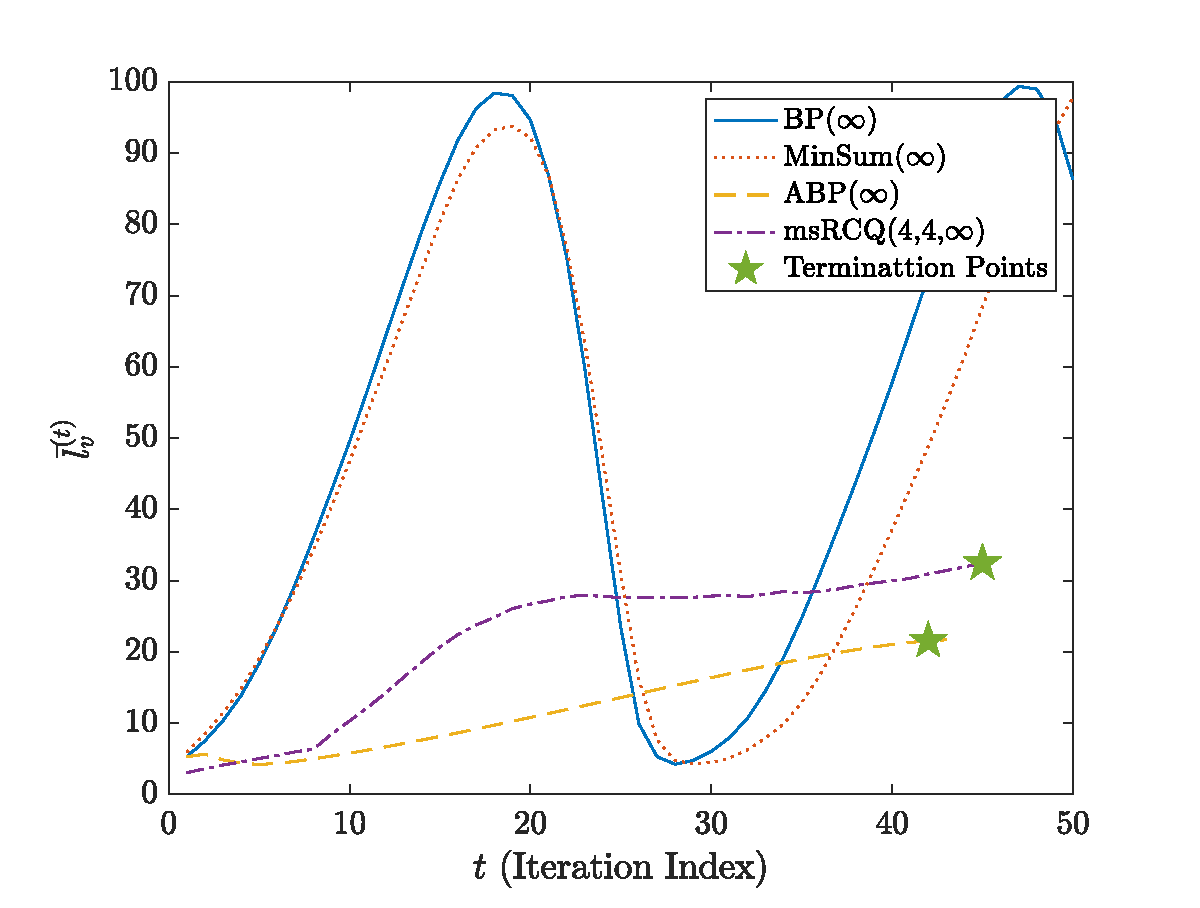
\includegraphics[width=0.5\linewidth]{figures/80211_fig2.eps}
	\caption{Average magnitudes of $l^{(t)}_v$ vs. iteration for BP, ABP, \minsum and msRCQ for Fig.  6a simulation at  $\frac{E_b}{N_o}=2.6$ dB.
	}
	\label{fig: 80211_2}
\end{figure}
As noted in \cite{ABP}, a possible indicator of the emergence of error trapping sets may be a sudden magnitude change in the values of certain variable node messages, or fast convergence to an unreliable estimate. Therefore, slowing down the convergence rate of VN messages can decrease the frequency of trapping set events. Both msRCQ decoder and A-BP in \cite{ABP} reduce the the convergence rate of VN messages and hence deliver a lower error floor. However, A-BP requires extra computations to calculate the average message. On the other hand, the averaging process of msRCQ (i.e., \ref{equ: ave_msrcq}) is inherent in $R(\cdot)$ and does not require additional complexity. 

The effect of averaging can be seen in Fig. \ref{fig: 80211_2}, which gives the average magnitude of $l^{(t)}_v$ for four decoders with a noise-corrupted all-zero codeword at $\frac{E_b}{N_o}=2.6$ dB as the input. The oscillation pattern of the BP decoder has been reported and discussed in \cite{ABP}.  As shown in Fig. \ref{fig: 80211_1}, ABP also outperforms belief propagation when $\frac{E_b}{N_o}$ is high. 
The oscillation occurs as errors alternate between the variable nodes that comprise the trapping set and their complement.
Note that ABP requires extra computations to calculate the average message. However, the implicit averaging process of msRCQ (i.e., \eqref{equ: ave_msrcq}) is inherent in $R(\cdot)$. 

Fig. \ref{fig: 80211_3} compares msRCQ(4,10) with other non-uniform quantization LDPC decoders. Simulation results show that both IB\cite{Lewandowsky2018-IBRegular} and Min-IB\cite{Meidlinger2017-MINIBIRR} decoders exhibit an error floor after $2.40dB$. The MIM-QMS\cite{kang2020generalized} decoder has a similar decoding structure to msRCQ. Note that MIM-QMS requires the determination of the internal bit width used by the VNs before designing quantization and reconstruction parameters, so reducing the bit width of VNs requires another design cycle. 
In contrast, for the purposes of HDQ discrete density evolution design process, msRCQ assumes that the internal VN  messages are real-valued. This assumption is an approximation since the internal VN messages will have finite precision in practical implementations. During actual decoding, the reconstruction operation $R(\cdot)$ produces a high-precision representation for use in computations at the VN. We found that assuming real-valued internal messages in the design process introduces negligible loss for practical internal message sizes while greatly simplifying the design. Our simulation results in \ref{fig: 80211_3} confirm that high precision internal messages have FER performance that is very close to real-valued internal messages.
Actually, for the msRCQ, it is sufficient to have a simple clipping module at variable node, because all reconstructed values are fixed point messages. 
The RCQ decoder has more efficient memory usage than LUT-based decoders. For the investigated non-uniform LDPC code, 4-bit IB and 4-bit Min-IB require 14.43k and 10.24k bits, respectively, for storing LUTs per iteration, whereas msRCQ(4,12) and msRCQ(4,10) require 165 bits and 135 bits only.   
\begin{figure}[t] 
    \centering
  \subfloat[\label{fig: 8k_FER}]{%
       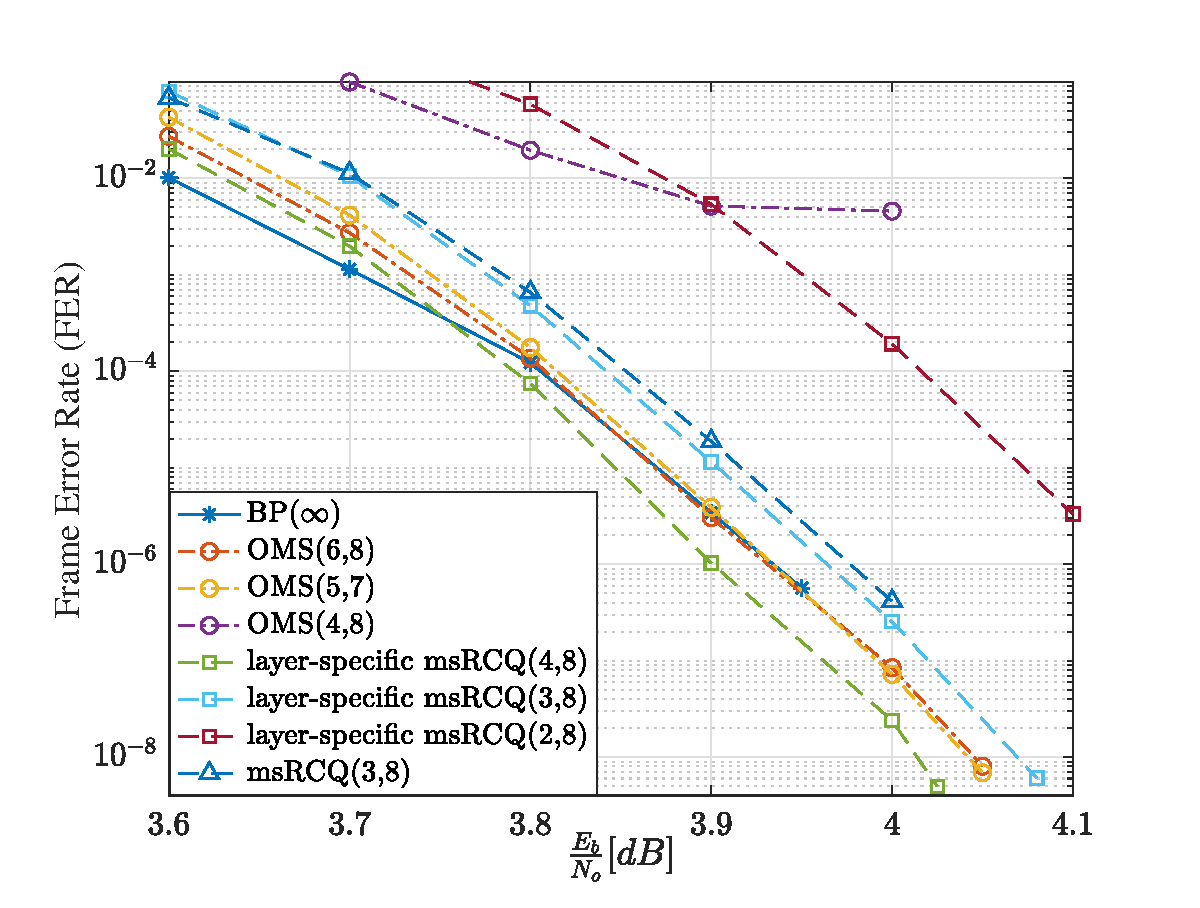
\includegraphics[width=0.5\linewidth]{figures/8k_fer3.eps}}
    \hfill
  \subfloat[\label{fig: 8k_ADIT}]{%
        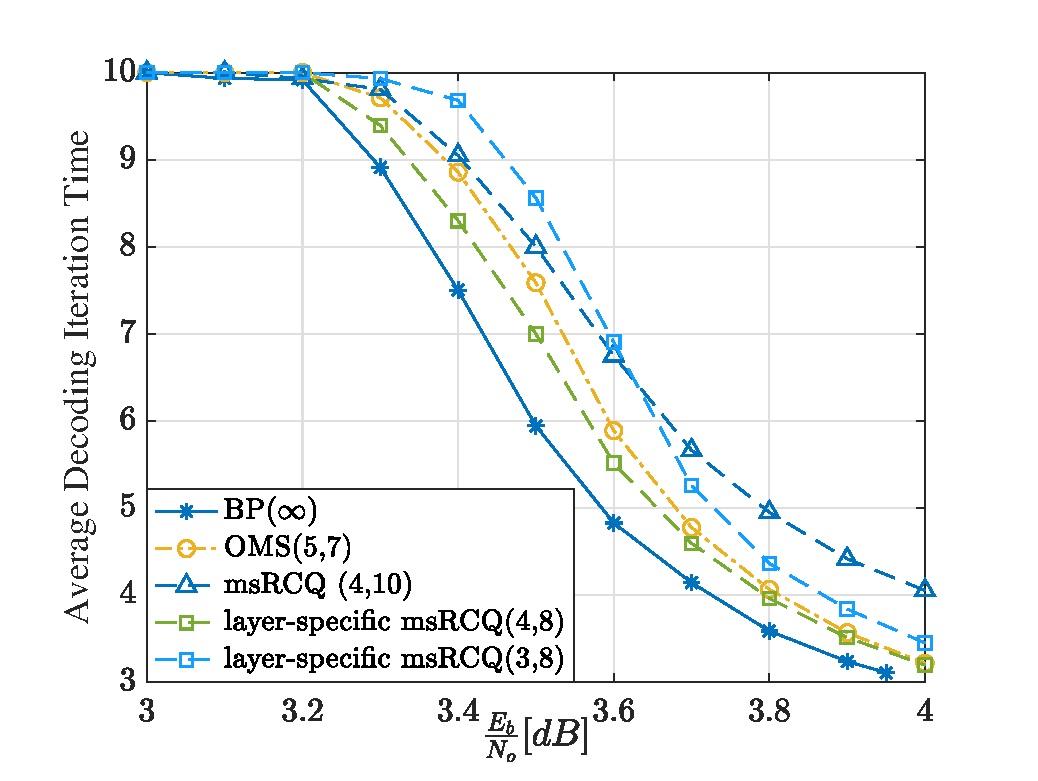
\includegraphics[width=0.5\linewidth]{figures/8K_ADIT.eps}}
  \caption{Fig. (a): FER performance of fixed point L-msRCQ decoders for (9472, 8192) LDPC code.  Fig.  (b): FER performance of fixed point L-msRCQ decoders for (9472, 8192) LDPC code. } \label{fig: 8k_performance}
\end{figure}

\subsection{(9472, 8192) QC-LDPC code}
In this subsection we consider a rate-0.8649 quasi-regular LDPC code, with all VNs having degree 4 and CNs having degree 29 and 30, as might be used in a flash memory controller. We study this (9472, 8192) QC-LDPC code using various decoders with a \textit{layered schedule}. The layer number of the investigated LDPC code is 10.  

Fig. \ref{fig: 8k_FER} shows the FER curves of various decoders. The maximum number of decoding iterations of all studied decoders is 10. The layer-specific msRCQ(4,8) outperforms msRCQ(4,10) by 0.04 dB, which shows the benefit of optimizing layer and iteration specific RCQ parameters.  
The layer-specific msRCQ(3,8) delivers similar decoding performance to msRCQ(4,10). The decoding performance of 2-bit layer-specific msRCQ has a 0.2 dB degradation compared with the 4-bit  layer-specific msRCQ decoder. 
Given that  $I_T=10$, the thresholds of the investigated LDPC code under 4-bits msRCQ and 2-4 bit LS-msRCQ decoders  are 3.58 dB, 3.67 dN,  3.46 dB  and 3.40 dB, respectively. 
Fig. \ref{fig: 8k_FER} also shows a fixed point offset \minsum (OMS) decoder with offset factor 0.5. At a FER of $10^{-8}$, OMS(6,8) and OMS(5,7) outperform layer-specific msRCQ(3,8) by 0.02 dB, yet are inferior to layer-specific msRCQ(4,8) by 0.02 dB.  
\begin{table*}[t]
    \centering
    \caption{\label{tab: hardware_usage_1} Hardware Usage of Various Decoding Structure for (9472,8192) QC-LDPC Code }
    \begin{tabular}{|c|c|c|c|c|}
    \hline
    Decoding Structure & LUTs                       & Registers                  & BRAMS                        & Routed Nets                \\ \hline
    OMS(5,7) (baseline)          & 21127                      & 12966                     & 17                    & 29202                      \\ \hline
    layer-specific RCQ(4,8)           & 20355(\textcolor{mygreen}{$\downarrow 3.6\%$} ) & 13967(\textcolor{red}{$\uparrow 7.0\%$}) & 17.5(\textcolor{red}{$\uparrow .03\%$}) & 28916(\textcolor{mygreen}{$\downarrow 1\%$}) \\ \hline
    layer-specific RCQ(3,8)           & 17865(\textcolor{mygreen}{$\downarrow 15.4\%$}) & 12098(\textcolor{mygreen}{$\downarrow 6.7\%$}) & 17(\textcolor{blue}{$-$})                &  25332\textcolor{mygreen}{($\downarrow 13.3\%$}) \\ \hline
    \end{tabular}
    \end{table*}
Fig. \ref{fig: 8k_ADIT} shows the average decoding iteration times for some of the decoders studied in Fig. \ref{fig: 8k_FER}. At high $\frac{E_b}{N_o}$, the msRCQ(4,10) decoder requires the largest average number of iterations to complete decoding. On the other hand, layer-specific msRCQ(4,8) has a similar decoding iteration time to OMS(5,7) and BP($\infty$) in this region. Layer-specific msRCQ(3,8) requires a slightly higher average number of iterations than layer-specific msRCQ(4,8) and OMS(5,7). 
%The decoding iteration time of OMS(6,8), L-msRCQ(4,8) and L-msRCQ(3,8) are 3.13, 3.20 and 3.44, respectively.

We implemented OMS and layer-specific msRCQ decoders with different bit widths on the programmable logic of a Xilinx Zynq UltraScale+ MPSoC device for comparison. Each design meets timing with a 500 MHz clock. The broadcast method described in \cite{Terrill2021-ec} is used for RCQ design. 
Table \ref{tab: hardware_usage} summarizes the hardware usage of each decoder. 
Simulation result shows that layer-specific msRCQ(4,8) has a similar hardware usage with OMS(5,7), and layer-specific msRCQ(3,8) has more than a $10\%$ reduction in LUTs and routed nets and more than a $6\%$ reduction in registers, compared with OMS(5,7).

\section{Conclusion}\label{sec: conclusion}
This chapter investigates the decoding performance and resource usage of RCQ decoders. For decoders using the flooding schedule, simulation results on an IEEE 802.11 LDPC code show that a 4-bit msRCQ decoder has a better decoding performance than LUT based decoders, such as IB decoders or Min-IB decoders, with significantly fewer parameters to be stored. It also surpasses belief propagation in the high $\frac{E_b}{N_o}$ region because a slower message convergence rate avoids trapping sets. For decoders using the layered schedule, conventional RCQ design leads to a degradation of FER performance and higher average decoding iteration time. Designing a layer-specific RCQ decoder, which updates parameters in each layer and iteration, improves the performance of a conventional RCQ decoder under a layered schedule.
Layer-specific HDQ discrete density evolution is proposed to design parameters for RCQ decoders with a layered schedule. FPGA implementations of RCQ decoders are used to compare the resource requirements of the decoders studied in this paper. 
Simulation results for a (9472, 8192) QC LDPC code show that a layer-specific \minsum RCQ decoder with 3-bit messages achieves a more than $10\%$ reduction in LUTs and routed nets and a more than $6\%$ register reduction while maintaining comparable decoding performance, compared to a 5-bit offset \minsum~decoder.

\chapter{RCQ LDPC Decoding with Degree-Specific Neural Edge Weights}
\section{Introduction}
Low-Density Parity-Check  (LDPC) codes \cite{GallagerPhD1963} have been implemented broadly, including in NAND flash systems and wireless communication systems. In practice, decoders for LDPC codes with low message bit widths are desired when considering the limited hardware resources on the field-programmable gate arrays (FPGAs) or application-specific integrated circuits (ASICs), such as area, routing capabilities, and power utilization. Unfortunately, low-bitwidth decoders with uniform quantizers typically suffer a large degradation in decoding performance\cite{Lee2005-RFQThorpe}. Recently, the non-uniformly quantized decoders  \cite{Planjery2012-FAID,Xiao2020-sb, Lewandowsky2018-IB,Stark2018-IBMA,Stark2019-IBPBRL,Lee2005-RFQThorpe,He2019-RFQCai, Wang2020-kh,terrill2021fpga,wang2022TCOMRCQ}  have shown to deliver excellent performance with very low message precision. One promising decoding paradigm is called reconstruction-computation-quantization (RCQ) decoder \cite{Wang2020-kh,terrill2021fpga,wang2022TCOMRCQ}. 
 
The node operation in an RCQ decoder involves a reconstruction function that allows high-precision message computation and a quantization function that allows low-precision message passing between nodes. Specifically, the reconstruction function, equivalent to a dequantizer,  maps the low-bitwidth messages received by a node to  high-bitwidth messages for computation. The quantization function quantizes the calculated high-bitwidth messages to low-bitwidth messages that will be sent to its neighbor nodes. 
 As shown in \cite{terrill2021fpga}, the 4-bit  layer-scheduled RCQ decoder can have a better decoding performance than the 6-bit uniformly quantized offset MinSum (OMS) decoder. 

 The excellent decoding performance of RCQ decoder comes from its dynamic quantizers and dequantizers that are updated in each layer and each iteration. However, for practical consideration, the dynamic quantizers and dequantizers mean more look-up tables (LUTs). What's worse, the LUTs required for storing quantizers and dequantizers may offset the LUTs saved by using low bit width to pass messages.  As reported in \cite{wang2022TCOMRCQ}, the 4-bit RCQ decoder has a similar LUT usage to the 5-bit OMS decoder for a (9472,8192) LDPC code. 

Recently, numerous works have been focused on enhancing the performance of message-passing decoders with the help of neural networks (NNs) \cite{Nachmani2016-bs,Lugosch2017-ed,Nachmani2017-qq,Nachmani2018-ra,Liang2018-lw,Wu2018-zr,Lugosch2018-gu,Lyu2018-nz,Xiao2019-kj,Deng2019-cf,Abotabl2019-wt,Buchberger2020-pf,Wang2020-fb,Lian2019-jh,nguyen2021neural}. 
%The neural network is created by unfolding the message passing operations of each decoding iteration \cite{Nachmani2016-bs}.
%Each decoding iteration is unfolded into two hidden layers which represent check node processing layer and variable node processing layer and each neuron represents a variable-to-check message or a check-to-variable message. 
Nachmani \textit{et al.} in \cite{Nachmani2016-bs} propose a  neural belief propagation (N-BP) decoder that assigns NN-learned multiplicative weights to the BP messages.
Nachmani \textit{et al.} and Lugosch \textit{et al.} in \cite{Nachmani2018-ra, Lugosch2017-ed,Nachmani2016-bs} assign dynamic weights to the messages in  normalized MinSum (NMS) and OMS decoder and propose the Neural NMS (N-NMS) and Neural OMS (N-OMS) decoder, respectively.


For the above neural decoders, each check-to-variable message and/or each variable-to-check message is assigned a distinct weight in each iteration.
These neural decoders are impractical for long-blocklength LDPC codes because the number of required parameters is proportional to the number of edges in the Tanner graph corresponding to the parity check matrix.  
One solution is to share the weights across iterations or edges in the Tanner graph, like in \cite{Nachmani2017-qq,Wang2020-fb,Abotabl2019-wt, Lian2019-jh}. However, these simple weight-sharing methods sacrifice decoding performance in different ways.
Besides, the precursor works of literature are mainly focused on the short-blocklength codes ($n<2000$), which may have resulted from the fact that the required memory for training neural decoders with long block lengths by using popular deep learning research platforms, such as Pytorch, is larger than the computation resources of the researchers. 
However, as demonstrated in \cite{Abotabl2019-wt,wang2021ISTC}, it is possible to train neural decoders by only using CPUs on personal computers for very long-blocklength codes if resources are handled more efficiently. 

\subsection{Contribution}
This paper combines the recent neural decoding with RCQ decoding paradigm and proposes a weighted RCQ (W-RCQ) decoder. Unlike RCQ decoder, whose quantizers/dequantizers  change in each layer and iteration, the W-RCQ decoder limits the number of quantizer/quantizer pairs to a very small number, for example, three. However, the W-RCQ decoder weights check-to-variable node messages using dynamic parameters optimized via a quantized NN (QNN). The proposed W-RCQ decoder uses fewer parameters than the RCQ decoder, requiring much fewer LUTs. 

The novelties and contributions of this paper are summarized as follows:  
\begin{itemize}
    \item \textit{Posterior Joint Training Method.} This paper identifies the gradient explosion issue when training neural LDPC decoders. A posterior joint training method is proposed in this paper to address the gradient explosion problem. Simulation results show that posterior joint training delivers a better decoding performance than simply clipping large-magnitude gradients to some threshold value.
     \item \textit{Node-Degree-Based Weight Sharing}. 
     This paper illustrates that the weight values of the N-NMS decoder are strongly related to check node degree, variable node degree, and iteration index. As a result, this paper proposes node-degree-based weight-sharing schemes that assign the same weight to the edges with the same check and/or variable node degree.
     \item \textit{Neural-2D-MinSum decoder}. By employing the node-degree-based weight-sharing schemes on the N-NMS and N-OMS decoder, this paper proposes the N-2D-NMS decoder and N-2D-OMS decoder. \emph{2D} represents for 2-dimensional and implies that the weights are shared based on two dimensions, i.e., check node degree and variable node degree.
     Simulation results on the (16200,7200) DVBS-2 LDPC code show that the N-2D-NMS decoder can achieve same decoding performance as N-NMS decoder. 
    \item  \textit{W-RCQ Decoder.} This paper proposes the W-RCQ decoding paradigm.  Our simulation result for a (9472,8192) LDPC code on a field-programmable gate array (FPGA) device shows that the 4-bit W-RCQ decoder delivers comparable FER performance but with much fewer hardware resources, compared with the 4-bit RCQ decoder and the 6-bit offset MinSum decoder.
\end{itemize}

\subsection{Organization}

The remainder of this paper is organized as follows: Section \ref{sec: effi_NNMS} derives the gradients for a flooding-scheduled N-NMS decoder and shows that the memory to calculate the gradients can be saved by storing the forward messages compactly. The derivations enable one to build and train the NNs for the neural decoders using programmable languages such as C++. The compact message format saves the required memory for training NNs. This section also describes the posterior joint training method that addresses the gradient explosion issue. Section \ref{sec: N-2D-NMS} illustrates the relationship between neural weights of N-NMS decoder and node degree. The node-degree-based weight-sharing scheme is presented in this section. This section also gives neural-2D-MinSum decoders. Section \ref{sec: W-RCQ} gives the W-RCQ decoding structure and describes how to train W-RCQ  parameters via a QNN. The simulation results are presented in Section \ref{sec: Simulation}, and Section \ref{sec: conclusion_c2} concludes our work. 

\section{Training Neural MinSum Decoders for Long Blocklength Codes}\label{sec: effi_NNMS}
For the neural network corresponding to a neural LDPC decoder, the number of neurons in each hidden layer equals the number of edges in the Tanner graph corresponded to the parity check matrix  \cite{Nachmani2016-bs}. For the popular NN platforms, such as PyTorch, each neuron requires a data structure that stores the value of the neuron, the gradient of the neuron, the connection of this neuron with other neurons, and so on. Hence, there is a huge memory requirement for PyTorch to train the neural decoders for long-blocklength LDPC codes. (difficult for researchers with limited resources usage)


The data structure used in PyTorch is useful and convenient for conventional deep neural network tasks but redundant to the neural LDPC decoders. One reason is that the neuron connections between hidden layers are repetitive and can be interpreted by the parity check matrix.
%As a result, the neural network can perform the back propagation by only knowing the parity check matrix, rather than recording how each neurons are connected between two hidden layers. 
This immediately reduces the required memory.  
This section uses N-NMS decoder as an example to show that the memory required to calculate gradients of neural MinSum decoders can be further reduced by storing the messages in forward propagation compactly.

\subsection{Forward Propagation of N-NMS Decoder}
Let $H\in\mathbb{F}_2^{n\times k}$ be the parity check matrix of an $(n,k)$ binary LDPC code, where $n$ is the codeword length and $k$ is dataword length. Denote $i^{th}$ variable node and $j^{th}$ check node by $v_i$ and $c_j$, respectively. 
%In each iteration, an NMS decoder uses the same constant value to scale all  check-to-variable node messages, whereas an N-NMS decoder assigns distinct multiplicative parameters for each check-to-variable message in each iteration.  
For the flooding-scheduled decoder, in the $t^{th}$ decoding iteration, N-NMS decoder updates the check-to-variable (C2V) message, $u^{(t)}_{c_j \rightarrow v_i}$, by: 
\begin{align}
     u^{(t)}_{c_i\rightarrow v_j} &= \beta^{(t)}_{(c_i,v_j)} \times  \prod_{v_{j'}\in \mathcal{N}(c_i)\setminus\{v_j\}} \text{sgn}\left(l^{(t-1)}_{v_{j'}\rightarrow c_{i}}\right)  \times  \min_{v_{j'}\in \mathcal{N}(c_i)\setminus\{v_j\}} \left|l^{(t-1)}_{v_{j'}\rightarrow c_{i}}\right|,
\end{align}

$\mathcal{N}(c_i)$ is the set of variable nodes that connect $c_i$ and 
$\bigl\{\beta^{(t)}_{(c_i,v_j)}|i\in\{1,\ldots k\},j\in\{1,\ldots n\}, \allowbreak H(i,j)=1, t\in\{1,\ldots, I_T\} \bigr\}$ is the set of  trainable parameters. $I_T$ represents the maximum iteration. The variable-to-check (V2C) message, $l^{(t)}_{v_i\rightarrow c_j}$, and posterior of each variable node, $l_{v_i}^{(t)}$, of N-NMS decoder in iteration $t$
 are calculated by:
\begin{align}
l^{(t)}_{v_j\rightarrow c_i} &=  l^{ch}_{v_j} + \sum_{c_{i'}\in \mathcal{N}(v_j)\setminus\{c_i\}} u^{(t)}_{c_{i'}\rightarrow v_j}, \label{equ: v2c_update}\\
l^{(t)}_{v_j} &= l^{ch}_{v_j} + \sum_{c_{i'}\in \mathcal{N}(v_j)} u^{(t)}_{c_{i'}\rightarrow v_j}.\label{equ: pos_update}
\end{align}
$\mathcal{N}(v_j)$ represents the set of the check nodes that are connected to $v_j$. $l^{ch}_{v_j}$ is the log likelihood ratio (LLR) of channel observation of $v_j$. The decoding process stops when all parity checks are satisfied or $I_T$ is reached. 

\subsection{Backward Propagation of N-NMS}
% This subsection derives the gradients for flooding-scheduled N-NMS decoder. The gradient derivation for flooding-scheduled OMS, layer-scheduled N-NMS and N-OMS can be calculated in a similar way.   
Before performing back propagation to calculate the gradients, define $\texttt{min1}^{t}_{c_i}$, $\texttt{pos1}^{t}_{c_i}$, $\texttt{min2}^{t}_{c_i}$ and $\texttt{pos2}^{t}_{c_i}$ as follows:
\begin{align}
    \texttt{min1}^{t}_{c_i} &= \min_{v_{j'}\in \mathcal{N}(c_i)} |l^{(t)}_{v_{j'}\rightarrow c_{i}}|, &
    \texttt{pos1}^{t}_{c_i} &= \argminB_{v_{j'}\in \mathcal{N}(c_i)} |l^{(t)}_{v_{j'}\rightarrow c_{i}}|.\label{equ: min1}\\
    \texttt{min2}^{t}_{c_i} &= \min_{v_{j'}\in \mathcal{N}(c_i)/\{\texttt{pos1}^{t}_{c_i}\}}|l^{(t)}_{v_{j'}\rightarrow c_{i}}|,&
    \texttt{pos2}^{t}_{c_i} &= \argminB_ {v_{j'}\in \mathcal{N}(c_i)/\{\texttt{pos1}^{t}_{c_i}\}}|l^{(t)}_{v_{j'}\rightarrow c_{i}}|\label{equ: pos}.
\end{align}
$\texttt{min1}^{t}_{c_i}$ is the minimum magnitude that $c_i$ receives in iteration $t$, and the minimum magnitude is provided by the variable node $\texttt{pos1}^{t}_{c_i}$. Similarly,  $\texttt{min2}^{t}_{c_i}$ is the second minimum magnitude that $c_i$ receives in iteration $t$, and the second minimum magnitude is provided by  $\texttt{pos2}^{t}_{c_i}$.

Let $J$ be some loss function for N-NMS neural network, for example, the multi-loss cross entropy in \cite{Nachmani2016-bs}. Denote the gradients of loss $J$ with respect to (w.r.t.) the trainable weights, the C2V message and V2C message by $\frac{\partial J}{ \partial \beta^{(t)}_{(c_i,v_j)}}$, $\frac{\partial J}{\partial u^{(t)}_{c_i\rightarrow v_j}}$, and $\frac{\partial J}{\partial l^{(t)}_{v_j \rightarrow c_i}}$, respectively.

In iteration $t$, $\frac{\partial J}{\partial u^{(t)}_{c_i \rightarrow v_j}}$ is updated as follows:
\begin{align}
\label{equ: update-c}
    \frac{\partial J}{\partial u^{(t)}_{c_i \rightarrow v_j}} = \frac{\partial J}{\partial l^{(t)}_{v_j}}+ \sum_{c_{i'}\in \mathcal{N}(v_j)\setminus\{c_i\}}\frac{\partial J}{\partial l^{(t)}_{ v_j\rightarrow c_{i'} }}.
\end{align}
$\frac{\partial J}{\partial \beta^{(t)}_{(c_i,v_j)}}$ is calculated using $\frac{\partial J}{\partial u^{(t)}_{c_i \rightarrow v_j}}$ by:
\begin{align}\label{equ: gradient_beta}
    \frac{\partial J}{\partial \beta^{(t)}_{(c_i,v_j)}} = \frac{u^{(t)}_{c_i \rightarrow v_j}}{\beta^{(t)}_{(c_i, v_j)}} \frac{\partial J}{\partial u^{(t)}_{c_i\rightarrow v_j}}.
\end{align}
Let $u^{(t)*}_{c_i\rightarrow v_j}=\frac{u^{(t)}_{c_i \rightarrow v_j}}{\beta^{(t)}_{(c_i, v_j)}}$. Note that $u^{(t)*}_{c_i\rightarrow v_j}$ is the output of check node Min operation, and hence can be calculated efficiently  by knowing ${\mathrm{sgn}}(l^{(t)}_{v_j\rightarrow c_i})$, $\texttt{min1}^{t}_{c_i}$, $\texttt{min2}^{t}_{c_i}$, $\texttt{pos1}^{t}_{c_i}$. To see this,
\begingroup
\allowdisplaybreaks
\begin{align}
    \text{sgn}(u^{(t)*}_{c_i \rightarrow v_j}) &=   \prod_{v_{j'}\in \mathcal{N}(c_i)/\{v_j\}} \text{sgn}(l^{(t-1)}_{v_{j'}\rightarrow c_{i}}), \\
    |{u^{(t)*}_{c_i \rightarrow v_j}}| &= 
     \left\{ \begin{array}{l l}  \texttt{min2}^{t}_{c_i}, &  \quad  \text{if }v_j =  \texttt{pos1}^{t}_{c_i}   \\  \texttt{min1}^{t}_{c_i}, &  \quad \text{otherwise} \\ \end{array}. \right.
\end{align}
\endgroup

For all variable nodes connected to check node $c_i$,  in iteration $t$, only $\texttt{pos1}^{(t)}_{c_i}$ and $\texttt{pos2}^{(t)}_{c_i}$ receive backward information. Hence, $\frac{\partial J}{\partial l^{(t-1)}_{v_j\rightarrow c_i}}$ is computed as follows:
\begin{align}
\label{equ: l_update}
    \frac{\partial J}{\partial l^{(t-1)}_{v_j\rightarrow c_i}} = \left\{ \begin{array}{l l} \text{sgn}\left(l^{(t-1)}_{v_j\rightarrow c_i}\right)\sum_{v_{j'}\in \mathcal{N}
    (c_i)\setminus \{v_j\}} \frac{\partial J}{\partial |{u^{(t)*}_{c_i \rightarrow v_{j'}}} |} & , v_j = \texttt{pos1}^{(t)}_{c_i}   \\ \text{sgn}\left(l^{(t-1)}_{v_j\rightarrow c_i}\right) \frac{\partial J}{\partial \left|{u^{(t)*}_{ c_i \rightarrow  \texttt{pos1}^{(t)}_{c_i}}} \right|}  &  , v_j = \texttt{pos2}^{(t)}_{c_i} \\  0 & , \text{otherwise}  . \\ \end{array} \right. 
\end{align} 
The term $\frac{\partial J}{\partial |{u^{(t)*}_{c_i \rightarrow v_j}} |}$ is calculated by:
\begin{align}\label{equ: end_back_prob}
    \frac{\partial J}{\partial |{u^{(t)*}_{c_i \rightarrow v_j}} |}= \text{sgn}(u^{(t)*}_{c_i \rightarrow v_j}) \beta_{(c_i,v_j)}^{(t)}\frac{\partial J}{\partial {u^{(t)}_{c_i \rightarrow v_j}} }.
\end{align}

\eqref{equ: update-c}-\eqref{equ: end_back_prob} indicate that the neuron values in each hidden layer can be stored compactly with sgn$\left(l^{(t)}_{v_j \rightarrow c_i}\right)$, $\texttt{min1}^{t}_{c_i}$, $\texttt{min2}^{t}_{c_i}$, $\texttt{pos1}^{t}_{c_i}$ and $\texttt{pos1}^{t}_{c_i}$. The compactly-stored neural values in the hidden layers leads to a significant memory reduction.  Besides,  \eqref{equ: update-c}, \eqref{equ: l_update} and \eqref{equ: end_back_prob} imply that $\frac{\partial J}{\partial {u^{(t)}_{c_i \rightarrow v_j}} }$ and $\frac{\partial J}{\partial l^{(t)}_{v_j\rightarrow c_i}}$  can be calculated iteratively.  
Hence, the memory to store the gradients in two consecutive hidden layers, rather than all hidden layers, is sufficient to perform back propagation and calculate $\frac{\partial J}{\partial \beta^{(t)}_{(c_i,v_j)}}$. Note that the compact message format \eqref{equ: min1}-\eqref{equ: pos} is also used in the hardware implementation for the MinSum decoders.

\subsection{Posterior Jointly Training}\label{Sec: gradient_explosion}
\begin{figure}[t] 
    \centering
  \subfloat[\label{fig: gradient_explosion}]{%
      \includegraphics[width=0.50\linewidth]{figures/Gradient_Explosion.pdf}}
    \hfill
  \subfloat[\label{fig: FER-FNNMS-1}]{%
        \includegraphics[width=0.50\linewidth]{figures/posterior_training.pdf}}
  \caption{Fig. (a): The average magnitude of gradients of loss $J$ w.r.t. C2V messages in each decoding iteration. The gradients are calculated by feeding the flooding-scheduled (3096,1032) N-NMS decoder with an input sample and performing backward propagation. Fig. (b): FER curves of the flooding-scheduled N-NMS decoders for a (3096,1032) LDPC code.  Gradient clipping, greedy training and posterior jointly training are used to address gradient explosion issue. The maximum decoding iteration is 50. The belief propagation decoder and NMS decoder with factor 0.7 are presented as comparison.}
\end{figure}
Equation \eqref{equ: l_update} implies that in iteration $t$, for all variable nodes that connect check node $c$, only $\texttt{pos1}_{c}^{t}$ and $\texttt{pos2}_{c}^{t}$ receive gradients from $c$. Besides, $|\mathcal{N}(c)|-1$ gradient terms flow to $\texttt{pos1}_{c}^1$. Hence, if check node  $c$ has a large degree, the gradient of $J$ w.r.t. $\texttt{pos1}_{c}^{t}$ can have a large magnitude, and this large-magnitude gradient will be propagated to the neurons in the preceding layer that corresponded to the C2V messages whose check nodes (other than $c$) connect $\texttt{pos1}_{c}^{t}$.  As a result, the large-magnitude gradients are accumulated and propagated as back propagation proceeds, which results in gradient explosion.

Fig. \ref{fig: gradient_explosion} shows the gradient explosion phenomenon when training a flooding-scheduled N-NMS decoder for a (3096,1032) LDPC code. Define $\mu^{(t)}$ as the average magnitude of the gradients of $J$ w.r.t. all C2V messages in iteration $t$. The gradients are calculated by feeding the  N-NMS decoder with some input sample and then performing backward propagation. Fig. \ref{fig: gradient_explosion} plots $\mu^{(t)}$ in each decoding iteration. The maximum check node degree and variable node degree of the code are 19 and 27, respectively. The maximum decoding iteration of the decoder is 50.  It can be seen that the $\mu^{(t)}$ increases exponentially with the decrease of decoding iteration $t$.

\eqref{equ: gradient_beta} indicates that  large magnitude of $\frac{\partial J}{\partial u^{(t)}_{(c,v)}}$ leads to large magnitude of $\frac{\partial J}{\partial \beta^{(t)}_{(c,v)}}$  and hence prevents the neural network from optimizing weights effectively. To the best of our knowledge, this paper is the first one to report the gradient explosion issue for neural LDPC decoder training. However, there have been several techniques that solve the gradient explosion problem:

\begin{enumerate} 
    \item \textit{Gradient Clipping}. Gradient explosion is a common problem in the deep learning field such as recurrent neural network, and one way to solve this problem is gradient clipping \cite{GoodBengCour16}.  There are various methods for gradient clipping \cite{mikolov2012, Pascanu2013-es}. This paper considers to  simply limit the maximum gradient magnitude to be some threshold $l$.
    
    \item \textit{Greedy Training}. Dai \textit{et al} in \cite{dai2021learning} proposed greedy training. Greedy training trains the parameters in $t^{th}$ decoding iteration by fixing the pre-trained parameters in the first $t-1$ iterations. Greedy training solves the gradient explosion problem because the large magnitude gradients won't be accumulated and propagated to the preceding hidden layers, i.e, decoding iterations. 
    However, greedy training requires a time complexity that is proportional to $I_T^2$, because one must have trained the $(t-1)$-iterations decoder in order to train
    a $t$-iterations decoder.
\end{enumerate}

\eqref{equ: update-c} indicates that the gradient of $J$ w.r.t. $u^{(t)}_{c_i\rightarrow v_j}$ comes from two parts: the first part is from the posterior $l^{(t)}_{v_j}$, and the second part is from the V2C messages $l^{(t)}_{v_j\rightarrow c_i'}$, $c_{i'}\in \mathcal{N}(v_j) \setminus \{c_i\}$. Based on the previous analysis, if any $l^{(t)}_{v_j\rightarrow c_i'}$, $c_{i'}\in \mathcal{N}(v_j) \setminus \{c_i\}$ has a large magnitude gradient, the neuron $u^{(t)}_{c_i\rightarrow v_j}$  can also have a large magnitude gradient. This will result in a large magnitude to the gradient of $J$ w.r.t. $\beta^{(t)}_{(c_i,v_j)}$, as indicated by \eqref{equ: gradient_beta}.  In this paper, we propose posterior jointly training which calculates the gradient of $J$ w.r.t. $u^{(t)}_{c_i\rightarrow v_j}$ only using the posterior $l^{(t)}_{v_j}$.  More explicitly, for the flooding-scheduled  N-NMS neural network, $\frac{\partial J}{\partial u^{(t)}_{c_i\rightarrow v_j}}$ is calculated by:
\begin{align}\label{equ: pt_flooding}
         \frac{\partial J}{\partial u^{(t)}_{c_i \rightarrow v_j}} = \frac{\partial J}{\partial l^{(t)}_{v_j}}.
\end{align}
Hence,  the gradient of $J$ w.r.t. $\beta^{(t)}_{(c_i,v_j)}$ is calculated as:
\begin{align}\label{equ: gradient_beta_2}
    \frac{\partial J}{\partial \beta^{(t)}_{c_i \rightarrow v_j}} = \frac{u^{(t)}_{c_i \rightarrow v_j}}{\beta^{(t)}_{c_i\rightarrow v_j}} \frac{\partial J}{\partial u^{(t)}_{c_i\rightarrow v_j}}=\frac{u^{(t)}_{c_i \rightarrow v_j}}{\beta^{(t)}_{c_i\rightarrow v_j}}\frac{\partial J}{\partial l^{(t)}_{v_j}}.
\end{align}

By calculating the gradients of neurons in the $t^{th}$ decoding iteration only using   $l^{(t)}$, i.e., the posteriors in the $t^{th}$ decoding iteration, \eqref{equ: pt_flooding} and \eqref{equ: gradient_beta_2} prevent the large magnitudes that are due to  $\frac{\partial J}{\partial l^{(t)}_{ v_j\rightarrow c_{i'} }}$ from propagating to the preceding hidden layers. This idea resembles the greedy training method. However, the posterior jointly training optimizes parameters of all decoding iterations  jointly, hence it requires a time complexity that is proportional to $I_T$. 
    
For the layer-scheduled N-NMS decoder, the conventional back propagation calculates the gradient of $J$ w.r.t.  $ u^{(t)}_{c_i \rightarrow v_j}$ by:
\begin{align}\label{equ: conv_layer}
    \frac{\partial J}{\partial u^{(t)}_{c_i \rightarrow v_j}} =  \frac{\partial J}{\partial l^{(t)}_{v_j}}+ \sum_{\{i'|c_{i'}\in\mathcal{N}(v_j),i'>i\}}\frac{\partial J}{\partial l^{(t)}_{v_j \rightarrow c_{i'}}}+\sum_{\{i'|c_{i'}\in\mathcal{N}(v_j),i'<i\}}\frac{\partial J}{\partial l^{(t+1)}_{v_j \rightarrow c_{i'}}}.
\end{align}
Posterior jointly training abandons the last term in \eqref{equ: conv_layer} and calculates $\frac{\partial J}{\partial u^{(t)}_{c_i\rightarrow v_j}}$ as follows:
\begin{align}\label{equ: pt_layer}
    \frac{\partial J}{\partial u^{(t)}_{c_i \rightarrow v_j}} =  \frac{\partial J}{\partial l^{(t)}_{v_j}}+ \sum_{\{i'|c_{i'}\in\mathcal{N}(v_j),i'>i\}}\frac{\partial J}{\partial l^{(t)}_{v_j \rightarrow c_{i'}}}.
\end{align}
Fig. \ref{fig: FER-FNNMS-1} shows the frame error rate (FER) of flooding-scheduled N-NMS decoders for a (3096,1032) LDPC code. The maximum decoding iteration time is 50. All three methods are implemented for preventing gradient explosion. Especially, for the gradient clipping,  the threshold for gradient magnitude is $l=10^{-3}$. The performance of BP and NMS with the same decoding schedule and maximum decoding iteration are also given for comparison. The NMS decoder uses multiplicative factor 0.7. The simulation result shows that greedy training and posterior jointly training deliver a better better performance than simple gradient clipping method. Greedy training and posterior jointly training deliver a  similar performance, both of which are 0.4 dB better than conventional  NMS decoder and have a better performance than BP at 1.6 dB. However,  posterior jointly training has a lower time complexity than greedy training.

\section{Node-Degree-Based Weight Sharing}\label{sec: N-2D-NMS}

N-NMS and N-OMS decoder for the long-blocklength LDPC codes are impractical, because the number of parameters of these decoders is proportional to the number of edges in the corresponding Tanner graph. Weight sharing \cite{xie2021weight} solves this problem by assigning one weight to different neurons in the NN. Different weight sharing schemes have been proposed to reduce the number of neural weights in N-NMS and N-OMS decoder. However, simple weight sharing schemes, such as across iterations or edges in \cite{Wang2020-fb,Lian2019-jh}, degrade the decoding performance in different degrees. 

This section proposes node-degree-based weight sharing schemes which assign the same weights to the edges that have same check and/or variable node degree. We call the N-NMS and N-OMS decoder with node-degree-based weight sharing schemes by neural 2-dimensional NMS (N-2D-NMS) and neural 2-dimensional OMS (N-2D-OMS) decoder, respectively,  because they are similar to the 2D-MS decoders in \cite{Juntan_Zhang2005-2dnms,2doms}. Simulation results in Section \ref{sec: Simulation} show that N-2D-NMS decoder can deliver the same decoding performance with N-NMS decoder.

\subsection{Motivation}
In this subsection, we investigate the relationship between the neural weights of a flooding-scheduled N-NMS decoder and node degrees. 
The N-NMS decoder is trained for a  (3096, 1032) LDPC code, the same one used in Section  \ref{Sec: gradient_explosion}. The maximum decoding iteration is 10.
\begin{figure}[t]
    \centering
  \subfloat[\label{fig: mean-t}]{%
       \includegraphics[width=0.50\linewidth]{figures/beta_mean_vs_iteration.pdf}}
    \hfill
  \subfloat[\label{fig: degree-19-iter4}]{%
        \includegraphics[width=0.50\linewidth]{figures/weight_vn.pdf}}
  \caption{Mean values of messages of a flooding-scheduled N-NMS decoder for a (3096,1032) LDPC code in each iteration show strong correlations to check and variable node degree.}
   \label{fig: weights_evaluation}
\end{figure}

Define the set of neural weights of N-NMS decoder that are associated to check node degree $d_c$ in the $t^{th}$ decoding iteration by $\mathcal{B}^{(t,d_c)}$, and $\mathcal{B}^{(t,d_c)}=\{\beta^{(t)}_{(c_i,v_j)}|\text{deg}(c_i) = d_c\}$. Let $\bar{\beta}^{(t,d_c)}$ be the mean value of $\mathcal{B}^{(t,d_c)}$. Fig.\ref{fig: mean-t} shows $\bar{\beta}^{(t,d_c)}$ versus decoding iteration $t$ with all possible check node degrees. The simulation result shows a clear relationship between check node degree and $\bar{\beta}^{(t,d_c)}$, i.e. a larger check node degree corresponds to a smaller $\bar{\beta}^{(t,d_c)}$. This difference is significant in the first few iterations.
Additionally, $\bar{\beta}^{(t,d_c)}$ changes drastically in first few iterations for all check node degrees. 

In order to explore the relationship between the weights and variable node degrees given a check node degree $d_c$ and decoding iteration index $t$, we further define $ \mathcal{B}^{(t,d_c,d_v)}=\{\beta^{(t)}_{(c_i,v_j)}\allowbreak| \text{deg}(c_i)=d_c,\text{deg}(v_i)=d_v\}$. We denote  the average value of $\mathcal{B}^{(t,d_c,d_v)}$ by $\bar{\beta}^{(t,d_c,d_v)}$. Fig.\ref{fig: degree-19-iter4} gives the average weights corresponding to various check and variable node degrees at iteration $4$. Statistical results show that, given a specific iteration $t$ and check node degree $d_c$, a larger $d_v$ indicates a smaller $\bar{\beta}^{(t,d_c,d_v)}$. 

In conclusion, the weights of N-NMS decoder are correlated with check node degree, variable node degree, and decoding iteration index. Thus, node degrees should affect the weighting of messages on their incident edges when decoding LDPC codes. This observation motivates us to propose a family of N-2D-MS decoders in this paper. 
\begin{center}
    % Please add the following required packages to your document preamble:
% \usepackage{multirow}

\begin{table}[t]
    \centering
    \small
    \caption{Various Node-Degree-Based Weight Sharing Schemes and Required Number of Parameters per Iteration for Two Example Codes}
    \begin{tabular}{|c|c|c|c|c|}
    \hline
    \multirow{2}{*}{Type} & \multirow{2}{*}{$\beta^{(t)}_{*}$}                                    & \multirow{2}{*}{$\alpha^{(t)}_{*}$}                & \multicolumn{2}{c|}{\begin{tabular}[c]{@{}c@{}}The Number of Required\\  Parameters per Iteration\end{tabular}}                        \\ \cline{4-5} 
                          &                                                                       &                                                    & (16200,7200) DVBS-2 code & (3096,1032)  PBRL code \\ \hline
    \multicolumn{5}{|c|}{No Weight Sharing\cite{Nachmani2016-bs}}                                                                                                                                                                                                                                                     \\ \hline
    $0$            & $\beta^{(t)}_{(c_i,v_j)}$                                             & 1                                                  & $4.8*10^5$                                                          & $1.60*10^4$                                                      \\ \hline
    \multicolumn{5}{|c|}{Weight Sharing Based on Node Degree}                                                                                                                                                                                                                                   \\ \hline
    1                     & $\beta^{(t)}_{(\text{deg}{(c_i)},\text{deg}{(v_j)})}$                                 & 1                                                  & 13                                                                  & 41                                                               \\ \hline
    2                     & $\beta^{(t)}_{(\text{deg}{(c_i)})}$                                          & $\alpha^{(t)}_{(\text{deg}{(v_j)})}$                      & 8                                                                   & 15                                                               \\ \hline
    3                     & $\beta^{(t)}_{(\text{deg}{(c_i)})}$                                          & 1                                                  & 4                                                                   & 8                                                                \\ \hline
    4                     & 1                                                                  & $\alpha^{(t)}_{(\text{deg}{(v_j)})}$                      & 4                                                                   & 7                                                                \\ \hline
    \multicolumn{5}{|c|}{Weight Sharing Based on Protomatrix}                                                                                                                                                                                                                                   \\ \hline
    5\cite{dai2021learning}          & $\beta^{(t)}_{\left( \floor{\frac{i}{f}},\floor{\frac{j}{f}}\right)}$ & 1                                                  & $-$                                                                 & 101                                                              \\ \hline
    6                     & $\beta^{(t)}_{\left( \floor{\frac{i}{f}}\right)}$                     & 1                                                  & $-$                                                                 & 17                                                               \\ \hline
    7                     & 1                                                                       & $\alpha^{(t)}_{\left( \floor{\frac{j}{f}}\right)}$ & $-$                                                                 & 25                                                               \\ \hline
    \multicolumn{5}{|c|}{Weight sharing based on Iteration  \cite {Lian2019-jh,Abotabl2019-wt}}                                                                                                                                                                                                          \\ \hline
    8                     & $\beta^{(t)}$                                                         & 1                                                  & 1                                                                   & 1                                                                \\ \hline
    \end{tabular}\label{tab:weight_sharing}
    \end{table}
\end{center}
\subsection{Neural 2D Normalized MinSum Decoders}
Based on the previous discussion, it is intuitive to consider assigning the same weights to messages with same check node degree and/or variable node degree. 
In this subsection, we propose a family node-degree-based weight sharing schemes.
These weight sharing schemes can be used on the  N-NMS decoder, which gives N-2D-NMS decoder. 

In the $t^{th}$ iteration, a flooding-scheduled N-2D-NMS decoder update $u^{(t)}_{c_i\rightarrow v_j}$ as follows:
\begingroup
\allowbreak
\begin{align}
     u^{(t)}_{c_i\rightarrow v_j} &= \beta^{(t)}_{*} \times  \prod_{v_{j'}\in \mathcal{N}(c_i)/\{v_j\}} \text{sgn}\left(l^{(t-1)}_{v_{j'}\rightarrow c_{i}}\right)  \times  \min_{v_{j'}\in \mathcal{N}(c_i)/\{v_j\}} \left|l^{(t-1)}_{v_{j'}\rightarrow c_{i}}\right|.\\
      l^{(t)}_{v_j\rightarrow c_i} &=  l^{ch}_{v_i} + \alpha^{(t)}_{*}  \sum_{c_{i'}\in \mathcal{N}(v_j)/\{c_i\}} u^{(t)}_{c_{i'}\rightarrow v_j},\\
    l^{(t)}_{v_j} &=  l^{ch}_{v_i} + \alpha^{(t)}_{*}  \sum_{c_{i'}\in \mathcal{N}(v_j)} u^{(t)}_{c_{i'}\rightarrow v_j}.
\end{align}
\endgroup



$\beta^{(t)}_{*}$ and $\alpha^{(t)}_{*}$ are the learnable weights. The subscript * is replaced in Table \ref{tab:weight_sharing} with the information needed to identify the specific weight depending on the weight sharing methodology. 
Table \ref{tab:weight_sharing} lists different weight sharing types, each identified in the first column by a type number. As a special case, we denote type 0 by assigning distinct weights to each edge, i.e., N-NMS decoder. Columns 2 and 3 describe how each type assigns $\beta^{(t)}_{*}$ and $\alpha^{(t)}_{*}$, respectively. In this paper, we refer to a decoder that uses a type-$x$ weight sharing scheme as a type-$x$ decoder. 

Types 1-4 assign the same weights based on node degree. In particular, Type 1 assigns the same weight to the edges that have same check node \emph{and} variable node degree. Type 2 considers the check node degree and variable node degree separately. As a simplification, type 3 and type 4 only consider check node degree and variable node degree, respectively.

Dai. \emph{et. al} in \cite{dai2021learning} studied weight sharing based on the edge type of multi-edge-type (MET)-LDPC codes, or protograph-based codes. We also consider this metric for types 5, 6, and 7. Type 5  assigns the same weight to the edges with the same edge type, i.e., the edges that belong to the same position in protomatrix. In Table. \ref{tab:weight_sharing}, $f$ is the lifting factor.  Types 6 and 7 assign parameters based only on the horizontal (protomatrix row) and vertical layers (protomatrix column), respectively.
Finally, type 8 assigns a single weight to all edges in each decoding iteration, as in \cite{Lian2019-jh,Abotabl2019-wt}. 

A (3096,1032) LDPC code and the (16200,7200) DVBS-2\cite{noauthor_2019-nv} standard LDPC code are considered in this section, and the number of parameters per iteration required for various weight sharing schemes of these two codes are listed in column 4 and 5 in Table. \ref{tab:weight_sharing}, respectively. It is shown that the number of parameters required by the node-degree-based weight sharing is less than that required by the protomatrix-based weight sharing.

\subsection{Neural 2D Offset MinSum Decoder}
The node-degree-based weight sharing schemes can be applied to N-OMS decoder in a similar way and lead to neural 2D OMS (N-2D-OMS) decoder. Specifically, a flooding N-2D-OMS decoder updates  $u^{(t)}_{c_i\rightarrow v_j}$ by: 
\begin{align}
     u^{(t)}_{c_i\rightarrow v_j} &= \prod_{v_{j'}\in \mathcal{N}(c_i)/\{v_j\}} \text{sgn}\left(l^{(t-1)}_{v_{j'}\rightarrow c_{i}}\right)  \times   \text{ReLu} \left(\min_{v_{j'}\in \mathcal{N}(c_i)/\{v_j\}} \left|(l^{(t-1)}_{v_{j'}\rightarrow c_{i}})\right|-\beta^{(t)}_*-\alpha ^{(t)}_*\right).
\end{align}
${\mathrm{ReLu}}(x)=\max(0,x)$. The $l_{v_j\rightarrow c_i}^{(t)}$ and $l_{v_j}^{(t)}$ are updated using \eqref{equ: v2c_update} and \eqref{equ: pos_update}. For the N-2D-OMS decoders, the constant value 1 in Table \ref{tab:weight_sharing} should be replaced by 0. 

\subsection{Hybrid Neural Decoder}
To further reduce the number of parameters, we consider a hybrid training structure that utilizes a neural network combining a feed forward module with a recurrent module. The corresponding decoder uses distinct neural weights for each of the first $I'$ decoding iterations and uses the same weights 
for the remaining  $I_T-I'$ iterations.
The motivation for the hybrid decoder is from the observation that the neural weights of N-NMS decoder change drastically in the first few iterations, but negligibly during the last few iterations, as illustrated in Fig. \ref{fig: weights_evaluation}. Therefore, using the same parameters for the last few iterations doesn't cause a large performance degradation. 

\section{Weighted RCQ Decoder}\label{sec: W-RCQ}
This section combines the N-2D-NMS or N-2D-OMS decoder with RCQ decoding paradigm and proposes a weighted RCQ (W-RCQ) decoder. Unlike the RCQ decoder, whose quantizers and de-quantizers are updated in each iteration (and each layer, if layer-scheduled decoding is considered), W-RCQ decoder only uses a small number of quantizers and dequantizers during the decoding process. However, the C2V messages of W-RCQ decoder will be weighted by dynamic node-degree-based parameters that that are trained by a QNN.
\begin{figure}[t]
	\centering
	\includegraphics[width=20pc]{figures/neural_rcq.pdf}
	\caption{Layer-scheduled Neural Offset RCQ Decoder Structure}
    \label{fig: layered_neural_RCQ_str}
\end{figure}
\subsection{Structure}
Fig. \ref{fig: layered_neural_RCQ_str} gives the decoding paradigm of a layer-scheduled weighted OMS-RCQ decoder (W-OMS-RCQ).
The offset parameters in Fig. \ref{fig: layered_neural_RCQ_str}, $\beta^{(t)}_{({\mathrm{deg}}(c_i),{\mathrm{deg}}(v_j))}$, use type-1 weight sharing scheme in the Table \ref{tab:weight_sharing}. $b^c$ denotes the bit width of C2V message,  and $b^v$ denotes the bitwidth for V2C message and variable node posterior. 
$l_{v_j}$ is the posterior of variable node $v_j$. 
In the $t^{th}$ iteration, a layer-scheduled W-OMS-RCQ decoder calculates the messages $u^{(t)}_{c_i\rightarrow v_{j'}}$ and updates the posteriors $l_{v_{j'}}$ as follows: 
\begingroup
\allowdisplaybreaks
\begin{align}
     &{\tilde{l}}_{v_{j'} \rightarrow c_{i}} \leftarrow  l_{v_{j'}}-{\mathrm{Relu}}\left( R\left(u^{(t-1)}_{c_i\rightarrow v_{j'}}\right)-\beta^{(t-1)}_{({\mathrm{deg}}(c_i),{\mathrm{deg}}(v_{j'}))}\right),~~\forall j'\in\mathcal{N}(c_i),\\
     &{l}^{(t)}_{v_{j'}\rightarrow c_i} = Q\left(\tilde{l}^{(t)}_{v_{j'}\rightarrow c_i}\right),~~\forall j'\in\mathcal{N}(c_i),\\
    &u^{(t)}_{c_i\rightarrow v_{j'}} =
    \left(\prod_{\tilde{j}\in\mathcal{N}(c_i)\setminus\{{j'}\}}{\mathrm{sgn}}\left(l_{v_{\tilde{j}}\rightarrow c_i}\right)\right)\times \min_{\tilde{j}\in\mathcal{N}(c_i)/\{{j'}\}}\left|l_{v_{\tilde{j}}\rightarrow c_i}\right|,~~\forall j'\in\mathcal{N}(c_i), \\
    &l_{v_{j'}} \leftarrow  {\tilde{l}}_{v_{j'}\rightarrow c_i}+{\mathrm{Relu}}\left( R\left(u^{(t)}_{c_i\rightarrow v_{j'}}\right)-\beta^{(t)}_{(\text{deg}(c_i),\text{deg}(v_{j'}))}\right), ~~\forall j'\in\mathcal{N}(c_i).
\end{align}
\endgroup
The differences between W-RCQ decoder and RCQ decoder are:
\begin{itemize}
    \item \textit{Reconstruction and Quantization}. The reconstruction and quantization functions in a layer-scheduled RCQ decoder are dynamic, which means that the decoder updates $R(\cdot)$ and $Q(\cdot)$ in each decoding layer and iteration. Storing the quantizers and dequantizers of all layers and iteration in the local variable node units (VNUs) will cost large amount of LUTs, hence a central control unit is considered for storing and distributing the parameters to each VNU\cite{terrill2021fpga}. 
    On the other hand, the neural RCQ decoder only uses very few number of $R(\cdot)$ and $Q(\cdot)$ across all decoding iterations, for example, three or less. Besides, as will be seen in the next subsection, we require that the thresholds of quantizers and mapping values of dequantizers have the same values. Each $R(\cdot)$ and $Q(\cdot)$ are used for several iterations. Hence,  $R(\cdot)$ and $Q(\cdot)$ are possible to be stored locally in VNUs.
    \item \textit{Message adjustment}. W-RCQ decoder weights the reconstructed C2V messages with additive or multiplicative parameters, which result in W-OMS-RCQ and W-NMS-RCQ, respectively. As shown in Fig. \ref{fig: layered_RCQ_str}, a central control unit is used for storing and distributing the weights to VNUs.
\end{itemize}

\subsection{Non-Uniform Quantizer}
An important design choice for a W-RCQ decoder is  the selection of quantization and reconstruction (dequantization) function. The authors in \cite{wang2022TCOMRCQ} use discrete density evolution to design dynamic quantizers and dequantizers. In \cite{Zhang2014-ib}, Zhang \emph{et. al.} point that  the message magnitude of iterative LDPC decoders can exhibit exponential behavior as a function of the number of decoding iterations, and the decoding performance of a quantized decoder can be improved by allowing exponential growth magnitude.  For example,  the authors in \cite{Zhang2014-ib} propose a ($q$+1)-bit quasi-uniform quantizer that uses one extra bit to efficiently
increase the dynamic range of messages.
For the W-RCQ decoder, this paper considers the quantizer and dequantizer that can be parameterized by a power function. 

Let $Q(x)$ be a symmetric $b^c$-bit quantizer that features sign information and a magnitude quantizer $Q^*(|x|)$. The magnitude quantizer selects one of $2^{b^\text{c}-1}$ possible indices using the threshold values $\{\tau_0,\tau_1,\ldots,\tau_{\text{max}}\}$, where  $\tau_j=C\left(\frac{j}{2^{b^c-1}}\right)^{\gamma}$ for $j\in\{0,\ldots,2^{b^{c}-1}-1\}$ and $\tau_{\text{max}}$ is $\tau_{j_{\text{max}}}$ for $j_{\text{max}} = 2^{b^\text{c}-1}-1$.
Given an input $x$, which can be decomposed into sign part ${{\mathrm{sgn}}(x)}$ and magnitude part $|x|$, $Q^*(|x|)\in \mathbb{F}_2^{b^{\mathrm{c}}-1}$ is defined by:
\begin{align}
    {Q}^*(|x|)=\left\{\begin{matrix}
  j, &    \tau_j\leq|x|<\tau_{j+1}\\
  2^{b_c-1}-1, & |x|\geq \tau_{\mathrm{max}} 
 \end{matrix}\right.,
 \label{equ: 10}
 \end{align}
 where $0\leq j\le j_{\text{max}}$. Let $s(x)$ be the sign bit of $x$, which is defined as $s(x)=\mathbbm{1}(x<0)$, $Q(x)$ is defined as
$Q(x)=[s(x)~Q^*(|x|)]$. The set of thresholds of $Q^*(|x|)$ has a power-function form and is controlled by two parameters. The parameter $C$ confines the maximum magnitudes the quantizer can take, and $\gamma$ manipulates the non-uniformity of the quantizer. 
Specifically, if $\gamma=1$,  $Q(x)$ becomes a uniform quantizer.

Let $d\in\mathbb{F}_2^{b^c}$ be a $b^c$-bit message. $d$ can be represented as $[d^{\text{MSB}}\ \tilde{d}]$, where $d^{\text{MSB}}\in\{0,1\}$ indicates sign and $\Tilde{d}\in\mathbb{F}_2^{b^\text{c}-1}$ corresponds to magnitude. The magnitude reconstruction function ${R}^*(\tilde{d}) = C\left(\frac{\tilde{d}}{2^{b_c}-1}\right)^{\gamma}$,
and $R(d)=(-2d^{\mathrm{MSB}}+1)R^*(\tilde{d})$. Note that both the magnitude quantization function and magnitude reconstruction function use  $\{\tau_1,\ldots,\tau_{\text{max}}\}$ as their parameters. 

The number of  required quantizer/dequantizer pairs for W-RCQ decoder can vary under different circumstances. If the code has a small variable node degree and the bit width of the quantizer is not too low (for example, 4 bits), one quantizer/dequantizer pair is sufficient through all decoding iterations. However, if the variable node degree of the LDPC code is high, or the bit width of quantizer is very small, using one quantizer/dequantizer pair is not able to accommodate the range of messages in the decoding process while providing a fine enough resolution, and is likely to degrade decoding performance. Therefore, we consider to use multiple quantizer/dequantizer pairs, and each pair is used for several iterations.

\subsection{Training Quantized Neural Network}
In this paper, we use the multi-loss cross entropy as the loss function and use posterior jointly training to train the QNN that is associated to the W-RCQ decoder. 
The parameters of the quantizers and dequantizers are fixed before training the neural network.
One problem of QNN is that quantization functions results in zeros derivatives almost everywhere.
In this work, we use a straight through estimator (STE)\cite{Bengio2013-kn, Xiao2020-sb} in the backward propagation. 

\subsection{Fixed-Point W-RCQ decoder}
This paper uses the pair ($b^c$,$b^v$) to denote the bitwidth for fixed-point decoders, where $b^c$ is the bitwidth of C2V messages and $b^v$ is the bitwith of V2C messages and the posteriors of variable nodes. For the W-RCQ decoders,  the learnable parameters are first trained under a floating point message representation and then quantized to $b^v$ bits. 

\begin{table}[t]
    \centering
    \caption{LDPC Codes used for Simulation}
    \begin{tabular}{|c|c|l|}
    \hline
    Code & Rate & \multicolumn{1}{c|}{Edge distribution} \\ \hline
    \multicolumn{1}{|c|}{\begin{tabular}[c]{@{}c@{}}(16200,7200) \\DVBS-2 LDPC code\\\cite{noauthor_2019-nv}\end{tabular}} & $\frac{4}{9}$ & \begin{tabular}[c]{@{}l@{}}$\lambda(x)=2.06*10^{-5}+0.3703x+$\\$0.3333x^2+0.2963x^7$\\ $\rho(x)=0.1186x^3+0.3332x^4+$\\$0.4445x^5+0.1037x^6$\end{tabular} \\ \hline
    \begin{tabular}[c]{@{}c@{}}(9472,8192)\\ QC-LDPC code\\ \cite{wang2022TCOMRCQ}\end{tabular} & $\frac{8}{9}$ & \begin{tabular}[c]{@{}l@{}}$\lambda(x)=x^3$\\ $\rho(x)=0.3919x^{28}+0.6081x^{29}$\end{tabular} \\ \hline
    \begin{tabular}[c]{@{}c@{}}$k=1032$ \\ PBRL LDPC code\\\cite{cls_tool}\end{tabular} & $\frac{8}{9}, \frac{8}{10},\dots,\frac{8}{24}$ & \begin{tabular}[c]{@{}l@{}}$\lambda(x)=0.1190+0.7940x^4+0.0952x^5+$\\ $0.0556x^6+0.3095x^{12}+0.1270x^{16}+0.2143x^{26}$\\ $\rho(x)=0.0238x^2+0.0635x^3+0.0794x^4+$\\ $0.1905x^5+0.2222x^6+0.1270x^7+0.1429x^{17}+$\\ $0.1508x^{18}$\end{tabular} \\ \hline
    \end{tabular}\label{tab: code_info}
    \end{table}

\section{Simulation Result and Discussion}\label{sec: Simulation}
This section evaluates the performance of the N-2D-NMS decoder and the W-RCQ decoder for LDPC codes with different block lengths and code rates. The LDPC codes used in this section are listed in Table \ref{tab: code_info}. All the encoded bits are modulated by binary phase-shift keying (BPSK) and transmitted through a Additive White Gaussian Noise (AWGN) channel. 


\begin{figure}[t]
    \centering
    \subfloat[\label{fig: dvbs2-fer}]{%
        \includegraphics[width=0.50\linewidth]{figures/fig5_a.pdf}}
    \hfill
    \subfloat[\label{fig: dvbs2-fer2}]{%
        \includegraphics[width=0.50\linewidth]{figures/fig5_b.pdf}}
    \caption{ Fig. (a): The FER performance of
        the N-2D-NMS decoders with various weight sharing types for the (16200,7200) DVBS-2 LDPC code.
        Fig. (b): The FER performance of the hybrid type-2 N-2D-NMS decoder that uses distinct weights in the first 20 iterations and same weights in the remaining 30 iterations. Simulation result shows that the hybrid type-2 N-2D-NMS decoder has comparable decoding performance with the type-2 N-2D-NMS decoder that assigns distinct weights in each iteration.  }
\end{figure}

\begin{figure}[t] 
    \centering
 \subfloat[\label{fig: beta_iter}]{%
       \includegraphics[width=0.50\linewidth]{figures/Fig_6_a_beta_iter.pdf}}
  \hfill
  \subfloat[\label{fig: alpha_iter}]{%
        \includegraphics[width=0.50\linewidth]{figures/Fig_6_b_alpha_iter.pdf}}
  \caption{ The change of weights of the type-2 N-2D-NMS decoder for (16200, 7200) DVBS-2 LDPC code w.r.t. check node degree, variable node degree and iteration index.
  Specifically, Fig. (a) gives $\beta^{(t)}_{(\text{deg}({c_i}))}$ for all possible check node degrees in each decoding iteration $t$, Fig. (b) gives $\alpha^{(t)}_{(\text{deg}({v_j}))}$ for all possible variable node degrees in each decoding iteration $t$.}
\end{figure}

\subsection{(16200,7200) DVBS-2 LDPC code}
Fig. \ref{fig: dvbs2-fer} shows the FER performances of N-2D-NMS decoders with various weight sharing types for the (16200, 7200) DVBS-2 LDPC code. 
The FER performance of BP and NMS decoders are also given for comparison.  The single multiplicative weight of  NMS decoder is 0.88.
All of the decoders are flooding-scheduled and maximum decoding iteration is 50. 
It is shown that the N-NMS decoder (i.e., type-0 decoder) outperforms BP at $1.3$ dB with a lower error floor. The type-1 and 2 decoders, which share weights based on the check node and variable node degree, deliver even a slightly better decoding performance than N-NMS decoder.

Fig. \ref{fig: dvbs2-fer} also shows that the FER performance degrades if only considering to sharing weights w.r.t. check node degree (type-3) or variable node degree (type-4). Specifically, in this example, type-4 N-2D-NMS decoder outperforms type-3 N-2D-NMS decoder, because the variable node weights of investigated code have a larger dynamic range than check node weights, as shown in Fig. \ref{fig: beta_iter}, and \ref{fig: alpha_iter}. Fig. \ref{fig: beta_iter} and \ref{fig: alpha_iter} give the $\beta^{(t)}_{(\text{deg}({c_i}))}$ and $\alpha^{(t)}_{(\text{deg}({v_j}))}$ of type-2 N-2D-NMS decoder, which agree with our observation in the previous section; i.e., in each decoding iteration, larger degree node corresponds to a smaller value. Besides, as shown in Fig. \ref{fig: beta_iter} and \ref{fig: alpha_iter}, the  weights change negligibly after $20^{th}$ iteration. Thus, the hybrid type-2 N-2D-NMS decoder with $I'=20$ delivers similar performance to the full feed forward decoding structure, as shown in Fig. \ref{fig: dvbs2-fer2}. 

\begin{figure}[t] 
    \centering
  \subfloat[\label{fig: fer_8k_1}]{%
       \includegraphics[width=0.50\linewidth]{figures/Fig7_a_8k_1.pdf}}
    \hfill
  \subfloat[\label{fig: fer_8k_2}]{%
        \includegraphics[width=0.50\linewidth]{figures/Fig7_a_8k_2.pdf}}
  \caption{Fig. (a): FER performance of W-OMS-RCQ decoders, RCQ decoders, and 6-bit OMS decoder for a (9472, 8192) QC LDPC code. Fig. (b): FER performance of 3-bit W-OMS-RCQ decoders with two and three quantizer/dequantizer pairs. Simulation result shows that the W-OMS-RCQ decoder with two quantizer/dequantizer pairs has an error error floor at FER of $10^{-7}$. }
\end{figure}

% Please add the following required packages to your document preamble:
% \usepackage{multirow}
\begin{table}[t]
    \centering
    \caption {The Quantizer/Dequantizer pairs of W-OMS-RCQ decoder for (9472,8192) LDPC code}
    \label{tab: 8k_config}
    \begin{tabular}{|c|c|c|}
    \hline
     CN bitwidth             & Quantizer/Reconstruction Parameter & Corresponding Decoder Iteration \\ \hline
    4 bits                  & $C=7$, $\gamma=1.7$                                                                       & $1\sim10$                                                                        \\ \hline
    \multirow{3}{*}{3 bits} & $C_1=3$, $\gamma_1=1.3$                                                                     & $1\sim6$                                                                         \\ \cline{2-3} 
                            & $C_2=5$, $\gamma_2=1.3$                                                                    & $7\sim8$                                                                         \\ \cline{2-3} 
                            & $C_3=7$, $\gamma_3=1.3$                                                                      & $9\sim10$                                                                        \\ \hline
    \end{tabular}
    \end{table}

\subsection{(9472,8192) Quasi-Cyclic LDPC code}
This subsection designs 3-bit and 4-bit W-OMS-RCQ decoders  for a (9742,8192) quasi-cyclic (QC) LDPC code  and compares them with the fixed-point OMS decoder and RCQ decoders. All decoders in this subsection are layer-scheduled with maximum iteration 10. The quantizer/reconstruction parameters for the 3-bit and 4-bit W-OMS-RCQ decoder are given in Table. \ref{tab: 8k_config}.

Fig. \ref{fig: fer_8k_1} compares the FER performances of W-OMS-RCQ decoders with RCQ decoders and a 6-bit OMS decoder. The decoders in Fig. \ref{fig: fer_8k_1} are also implemented using an FPGA device (Xilinx Zynq
UltraScale+ MPSoC) the study of resource usage. Table \ref{tab: hardware_usage} lists the usage of lookup tables (LUTs), registers, block RAM (BRAM), and routed nets of various decoders. For the details of FPGA implementations of the decoders, we refer the readers to \cite{terrill2021fpga}. 

Simulation result shows the 6-bit OMS decoder has the best FER performance. The 4-bit W-OMS-RCQ decoder and 4-bit RCQ decoder have similar FER performance, which are inferior to the 6-bit OMS decoder by 0.015 dB. However, as shown in Table \ref{tab: hardware_usage}, the 4-bit W-OMS-RCQ decoder requires much less resources compared with the 4-bit RCQ decoder and the 6-bit OMS decoder. Compared to the 6-bit OMS decoder, the 3-bit W-OMS-RCQ and 3-bit RCQ decoder have a gap of 0.04 and 0.06 dB, respectively. More specifically, the 3-bit RCQ decoder has a similar LUT, BRAM and routed net usage to the 4-bit W-OMS-RCQ decoder. On the other hand, the 3-bit W-OMS-RCQ uses much fewer resource than the 4-bit W-OMS-RCQ decoder.


\begin{table}[t]
    \small
    \caption{\label{tab: hardware_usage} Hardware Usage of Various Decoding Structure for (9472,8192) QC-LDPC Code }
    \centering
    \begin{tabular}{|c|c|c|c|c|}
    \hline
    Decoding Structure  & LUTs                                            & Registers                                       & BRAMS                                           & Routed Nets                                     \\ \hline
    OMS(6,8) (baseline) & 21127                                           & 12966                                           & 17                                              & 29202                                           \\ \hline
    RCQ(4,8)          & 20355(\textcolor{mygreen}{$\downarrow 3.6\%$} ) & 13967(\textcolor{red}{$\uparrow 7.0\%$})        & 17.5(\textcolor{red}{$\uparrow .03\%$})         & 28916(\textcolor{mygreen}{$\downarrow 1\%$})    \\ \hline
    RCQ(3,8)          & 17865(\textcolor{mygreen}{$\downarrow 15.4\%$}) & 12098(\textcolor{mygreen}{$\downarrow 6.7\%$})  & 17(\textcolor{blue}{$-$})                       & 25332\textcolor{mygreen}{($\downarrow 13.3\%$}) \\ \hline
    W-OMS-RCQ(4,8)         & 17645(\textcolor{mygreen}{$\downarrow 16.5\%$} ) & 13297(\textcolor{red}{$\uparrow 2.6\%$}) & 17(\textcolor{blue}{$-$}) & 25361(\textcolor{mygreen}{$\downarrow 13.2\%$} )\\ \hline
    W-OMS-RCQ(3,8)         & 16306(\textcolor{mygreen}{$\downarrow 22.82\%$} ) & 12104(\textcolor{mygreen}{$\downarrow 6.65\%$}) & 17(\textcolor{blue}{$-$}) & 23252(\textcolor{mygreen}{$\downarrow 20.38\%$} )\\ \hline
    \end{tabular}
    \end{table}

Fig. \ref{fig: fer_8k_1} compares the FER performances of W-OMS-RCQ decoders with RCQ decoders and a 6-bit OMS decoder. The decoders in Fig. \ref{fig: fer_8k_1} are also implemented using an FPGA device (Xilinx Zynq
UltraScale+ MPSoC) the study of resource usage. Table \ref{tab: hardware_usage} lists the usage of lookup tables (LUTs), registers, block RAM (BRAM), and routed nets of various decoders. For the details of FPGA implementations of the decoders, we refer the readers to \cite{terrill2021fpga}. 

Simulation result shows the 6-bit OMS decoder has the best FER performance. The 4-bit W-OMS-RCQ decoder and 4-bit RCQ decoder have similar FER performance, which are inferior to the 6-bit OMS decoder by 0.015 dB. However, as shown in Table \ref{tab: hardware_usage}, the 4-bit W-OMS-RCQ decoder requires much less resources compared with the 4-bit RCQ decoder and the 6-bit OMS decoder. Compared to the 6-bit OMS decoder, the 3-bit W-OMS-RCQ and 3-bit RCQ decoder have a gap of 0.04 and 0.06 dB, respectively. More specifically, the 3-bit RCQ decoder has a similar LUT, BRAM and routed net usage to the 4-bit W-OMS-RCQ decoder. On the other hand, the 3-bit W-OMS-RCQ uses much fewer resource than the 4-bit W-OMS-RCQ decoder.

The 3-bit W-OMS-RCQ decoder in Fig. \ref{fig: fer_8k_1} uses three quantizers for three decoding phases. In the first 3 iteration, most messages have low magnitudes, hence a quantizer with small $C$ is required for a finer resolution to the low-magnitude values. However, the message magnitudes increase with the increase of decoding iteration. As a result, the quantizers with larger $C$ should be used correspondingly. Fewer quantizers may not accommodate the message magnitude growth in the decoding process and will result in performance degradation. For example, Fig. \ref{fig: fer_8k_2} considers a 3-bit W-OMS-RCQ decoder that uses two quantizer/dequantizer pairs, the first pair has $C_1=3$, $\gamma_1=1.3$ and is used for iteration $1\sim7$, the second pair has $C_2=5$, $\gamma_2=1.3$ and is used for iteration $8\sim10$. Simulation result shows that the 3-bit W-OMS-RCQ decoder that uses 2 quantizer/dequantizer pairs has an early error floor at FER of $10^{-7}$.
\begin{figure}[t]
	\centering
	\includegraphics[width=0.5\linewidth]{figures/Fig8_N2DNMS_PBRL.pdf}  
	\caption{FER performance of N-2D-NMS decoders with various weight sharing types for a (3096,1032) PBRL LDPC code compared with N-NMS (type 0) and NMS.}
    \label{fig: FER1}
\end{figure}

subsection{$k=1032$ Protograph-Based Raptor-Like code}

5G LDPC codes have the protograph-based raptor-like (PBRL) \cite{PBRL} structure which offers inherent rate-compatibility and excellent decoding performance. In this subsection, we examine the performance of N-2D-NMS decoders and W-RCQ decoders for a $k=1032$ PBRL LDPC code, whose supported rates are listed in Table \ref{tab:weight_sharing}.  The edge distribution of the lowest-rate code, which corresponds to the full parity check matrix, is also given in Table \ref{tab:weight_sharing}.  All the decoders in this subsection are layer-scheduled with maximum 10 decoding iterations. 




Fig. \ref{fig: FER1} shows the FER performance of  N-2D-NMS decoder with various weight sharing types for the PBRL code with lowest code rates $\frac{1}{3}$. As a comparison, the decoding performance of the N-NMS (type 0) decoder and the NMS decoder are also given. All of the decoders use floating-point message representation. The simulation results show that N-NMS decoder has a more than 0.5 dB improvement over the NMS decoder. N-2D-NMS decoders with weight sharing types 1-7  are also simulated. 
%The number of parameters of N-NMS and N-2D-NMS decoders in each iteration are presented in  
%The types 1, 2 and 5 have the same decoding performance as the N-NMS decoder, with parameter reduction by 99.7\%, 99.9\% and 99.3\%, respectively. 
Simulation result shows that the N-2D-NMS decoders with weight-sharing metrics based on check and variable node degree (i.e., type 1 and 2), or based on horizontal and vertical layer  (i.e., type 5) deliver lossless performance w.r.t. N-NMS decoder.  N-2D-NMS decoders with weight sharing types 4 and 6 have a degradation of around 0.05 dB compared with the N-NMS decoder.  N-2D-NMS decoders with weight sharing types 5 and 7 have a degradation of around 0.2 dB compared with the N-NMS decoder. Thus, for this (3096,1032) PBRL LDPC code of Fig. \ref{fig: FER1}, assigning weights based only on check nodes can gain more benefit than assigning weights only based on variable nodes.

\begin{figure}[t] 
    \centering
  \subfloat[\label{fig: pbrl_fer_1}]{%
       \includegraphics[width=0.50\linewidth]{figures/Fig_9_a_rate_13_12.pdf}}
    \hfill
  \subfloat[\label{fig: pbrl_fer_2}]{%
        \includegraphics[width=0.50\linewidth]{figures/Fig_9_a_rate_23_89.pdf}}
  \caption{FER performance of 4-bit W-RCQ decoders for $k=1032$ PBRL code with different code rates. The term "rate-specific" means to design distinct decoders for each code rate; The term "rate-compatible" means to train one decoder that matches all code rates. The 6-bit OMS decoder is given as comparison. }\label{fig: pbrl}
\end{figure}

Fig. \ref{fig: pbrl} gives the FER performance of fixed-point W-NMS-RCQ decoders for the $k=1032$ PBRL code with rate $\frac{1}{3}$, $\frac{1}{2}$, $\frac{2}{3}$ and $\frac{8}{9}$. The W-NMS-RCQ decoder assigns 4 bits to C2V message and 10 bits to V2C message. Two quantizer/dequantizer pairs are used for W-NMS-RCQ decoder across all investigated rates.
The first quantizer has $C_1=7$, $\gamma_2=1.7$ and is used for the first 7 iterations. The second quantizer has $C_2=10$, $\gamma_2=2.3$ and is used for last 3 iterations.
We use a 6-bit OMS decoder as benchmark, because we find it delivers a better decoding performance than the NMS decoder with same bit width.
Additionally, we didn't consider W-OMS-RCQ decoder for this code because the 4-bit W-OMS-RCQ decoder doesn't perform as well as the 4-bit W-NMS-RCQ decoder. 

We first consider the 4-bit W-NMS-RCQ decoder with type-1 weight sharing that assigns the same weight to the edges with same check and variable node degree.
The decoder is rate-specific; i.e., for each considered rate, a W-NMS-RCQ decoder is trained separately.
The simulation results shows that, targeting a FER of $10^{-6}$, the 4-bit rate-specific W-NMS-RCQ decoder outperforms the 6-bit OMS decoder with 0.1$\sim$ 0.15 dB for all considered code rates.

For the PBRL code, the proto-matrix of each possible rate is a sub-matrix of a base proto-matrix \cite{PBRL}. As shown in Table. \ref{tab:weight_sharing}, the type-5 weight sharing assigns the same weight to the edges that correspond to the same element in the proto-matirx. Hence, it is possible to use \emph{one} trained type-5 neural decoder to match different code rates. We refer to such decoder as a rate-compatible decoder. In \cite{dai2021learning}, the authors propose to training the rate-compatible decoder by using the samples from different code rates. 

Fig. \ref{fig: pbrl} shows the decoding performance of rate-compatible type-5 W-NMS-RCQ decoder. Simulation result shows that for the higher rate such as $\frac{2}{3}$ and $\frac{8}{9}$, the rate-compatible type-5 W-NMS-RCQ decoder has a similar decoding performance to the rate-specific type-1 W-NMS-RCQ decoder whose parameters for each rate  are separately designed.  However, for the lower rate such as $\frac{1}{3}$ and $\frac{1}{2}$, the rate-compatible type-5 W-NMS-RCQ decoder method doesn't deliver a decoding performance as well as rate-specific type-1 W-NMS-RCQ decoder.
Besides, considering the four rates in Fig. \ref{fig: pbrl}, the number of neural weights for rate-specific type-1 and rate-compatible type-5  W-NMS-RCQ decoder are 96 and 101, respectively.

\section{Conclusion}\label{sec: conclusion_c2}
This chapter proposes the W-RCQ decoder, a non-uniformly quantized decoder that delivers excellent decoding performance in the low-bitwidth regime.
%Compared with RCQ decoder, W-RCQ decoder uses fewer parameters and provides comparable decoding performance. 
Unlike RCQ decoder, which designs quantizer/dequantizer pairs for each layer and iteration, W-RCQ decoder only uses a small number of quantizer/dequantizer pairs and each one is responsible for several iterations. 
The W-RCQ decoder uses Min operation at check node, and the C2V messages are weighted by multiplicative or additive parameters, which induce W-NMS-RCQ and W-OMS-RCQ, respectively. 

For the neural decoders such as W-RCQ decoder and N-NMS decoder, assigning distinct weights to each edge in each decoding iteration is impractical for long-blocklength codes because of huge number of neural weights.
This paper proposes various node-degree-based weight sharing schemes with  lossless or lossy performance for the neural decoders, depending on whether the weight sharing considers both check and variable node degree or only one of them. 

Additionally, this paper discusses the issues when training neural LDPC decoders. First, training the neural LDPC decoders for long blocklength code using Pytorch or TensorFlow could raise memory issue. This paper shows that the memory for training neural MinSum decoders can be saved by storing feed-forward messages compactly. Second, this paper identifies gradient explosion problem in the neural decoder training and proposes a  posterior jointly training method that addresses this problem. 


\bibliographystyle{uclathes}
%\bibliographystyle{thesis}
\bibliography{bio.bib}    % bibliography references

\end {document}

